\documentclass[11pt]{article}

\usepackage[a4paper]{geometry}
\geometry{left=2.0cm,right=2.0cm,top=2.5cm,bottom=2.5cm}

% Chinese support
\usepackage{ctex}

% Math packages
\usepackage{amsmath,amsfonts,amssymb,amsthm,bm,mathrsfs,mathtools,breqn}

% Graphics and Colors
\usepackage{graphicx}
\usepackage{xcolor}
\usepackage{tikz}
\usetikzlibrary{arrows.meta,positioning}
\usepackage{pgfplots}
\pgfplotsset{compat=1.18}
\usepackage{circuitikz}
\graphicspath{{fig/}}

% Units
\usepackage{siunitx}

% Algorithms
\usepackage{algorithm}
\usepackage[noend]{algpseudocode}

% Layout and formatting
\usepackage{fancyhdr}
\usepackage[framemethod=TikZ]{mdframed}
\usepackage{fontspec}
\usepackage{fontsize}
\usepackage{adjustbox}
\usepackage{float}
\usepackage{multicol}
\usepackage{multirow}
\usepackage{pdfpages}
\usepackage{wrapfig}
\usepackage{subcaption}
\usepackage[inline]{enumitem}

% Tables
\usepackage{booktabs}
\usepackage{bigstrut,rotating}

% Listings
\RequirePackage{listings}

% Hyperlinks
\usepackage{hyperref}
\hypersetup{colorlinks=true,linkcolor=blue}

% Cross-referencing
\usepackage[capitalize]{cleveref}
\Crefname{section}{Section}{Sections}
\Crefname{table}{表格}{表格}
\crefname{table}{表格}{表格}
\Crefname{figure}{图片}{图片}
\crefname{figure}{图片}{图片}

% Listing settings
\definecolor{dkgreen}{rgb}{0,0.6,0}
\definecolor{gray}{rgb}{0.5,0.5,0.5}
\definecolor{mauve}{rgb}{0.58,0,0.82}

\lstset{
  frame=tb,
  aboveskip=3mm,
  belowskip=3mm,
  showstringspaces=false,
  columns=flexible,
  framerule=1pt,
  rulecolor=\color{gray!35},
  backgroundcolor=\color{gray!5},
  basicstyle={\small\ttfamily},
  numbers=none,
  numberstyle=\tiny\color{gray},
  keywordstyle=\color{blue},
  commentstyle=\color{dkgreen},
  stringstyle=\color{mauve},
  breaklines=true,
  breakatwhitespace=true,
  tabsize=3,
}

\setmainfont{Palatino Linotype}
\setCJKmainfont{SimSun}[BoldFont=SimHei, ItalicFont=KaiTi]
\setCJKsansfont{SimHei}
\setCJKmonofont{FangSong}
\punctstyle{kaiming}
% 偏好的几个字体, 可以根据需要自行加入字体ttf文件并调用

% Restore standard emphasis to avoid requiring an undefined environment (kaishu).
% The original redefinition used an environment `kaishu` which is not defined
% in a default ctex setup and causes compilation errors. Use \textit for
% emphasis which works across engines.
\renewcommand{\emph}[1]{\textit{#1}}

%改这里可以修改实验报告表头的信息
\newcommand{\experiName}{光电探测}
\newcommand{\supervisor}{王慧}
\newcommand{\name}{邓思豪}
\newcommand{\studentNum}{2023K8009909008}
\newcommand{\class}{3}
\newcommand{\group}{01}
\newcommand{\seat}{5}
\newcommand{\dateYear}{2025}
\newcommand{\dateMonth}{12}
\newcommand{\dateDay}{3}
\newcommand{\room}{西实206}
\newcommand{\others}{$\square$}


\begin{document}



\begin{center}
    \LARGE \bf 《\, 基\, 础\, 物\, 理\, 实\, 验\, 》\, 实\, 验\, 报\, 告
\end{center}

\begin{center}
    \noindent \emph{实验名称}\underline{\makebox[25em][c]{\experiName}}
    \emph{指导教师}\underline{\makebox[8em][c]{\supervisor}}\\
    \emph{姓名}\underline{\makebox[6em][c]{\name}} 
    % 如果名字比较长, 可以修改box的长度"6em"
    \emph{学号}\underline{\makebox[10em][c]{\studentNum}}
    \emph{分班分组及座号} \underline{\makebox[5em][c]{\class \ -\ \group \ -\ \seat }\emph{号}} （\emph{例}:\, 1\,-\,04\,-\,5\emph{号}）\\
    \emph{实验日期} \underline{\makebox[3em][c]{\dateYear}}\emph{年}
    \underline{\makebox[2em][c]{\dateMonth}}\emph{月}
    \underline{\makebox[2em][c]{\dateDay}}\emph{日}
    \emph{实验地点}\underline{{\makebox[6em][c]\room}}
    \emph{调课/补课} \underline{\makebox[3em][c]{\others\ 是}}
    \emph{成绩评定} \underline{\hspace{5em}}
    {\noindent}
    \rule[8pt]{17cm}{0.2em}
\end{center}

\section{实验目的}

\begin{enumerate}
    \item 理解硅光电池的工作原理，明确光生伏特效应的物理过程及 PN 结在光电转换中的作用；
    \item 掌握硅光电池在无光照射时的二极管伏安特性，以及光照强度不变时的负载特性测量方法；
    \item 学会通过实验数据计算硅光电池的短路电流（$I_{SC}$）、开路电压（$U_{OC}$）、最大输出功率（$P_m$）及填充因子（$FF$），理解这些参数的物理意义；
    \item 掌握实验数据的拟合与分析方法；
\end{enumerate}

\section{实验仪器与用具}


\begin{figure}[htbp]
     \centering
     
\includegraphics[width=0.6\textwidth]{fig1.png}
     \caption{实验机箱}
 \end{figure}

 \begin{figure}[htbp]
     \centering
     \begin{minipage}[t]{0.45\textwidth}
         \centering
         
\includegraphics[width=\textwidth]{fig2.png}
         \caption{机箱开盖图}
     \end{minipage}
     \hfill
     \begin{minipage}[t]{0.45\textwidth}
         \centering
         
\includegraphics[width=\textwidth]{fig3.png}
         \caption{内部结构示}
     \end{minipage}
 \end{figure}

本实验采用 \textbf{FD-SBC-B 型硅光电池特性测试实验仪}，配套设备包括实验连接线（红黑各 5 根），仪器核心结构与技术指标如下：

\subsection{仪器核心结构}

\begin{table}[htbp]
    \centering
    \begin{tabular}{|c|p{10cm}|}
        \hline
        \textbf{部件名称} & \multicolumn{1}{c|}{\textbf{功能说明}} \\ \hline
        光源模块 & 射灯型结构，提供实验所需的可变强度光源，光源位置可通过支架与导轨调节。 \\ \hline
        硅光电池盒 & 内置硅光电池与光功率计（位于电池盒两侧），用于接收光照并测量光强，通过滑块固定在导轨上，可调节与光源的距离。 \\ \hline
        电路模块 & 包含稳压电源（$0-9.0\,\text{V}$）、变阻器（$0-100\,\text{k}\Omega$）、取样电阻（$1\,\text{k}\Omega$、$10\,\text{k}\Omega$、$100\,\text{k}\Omega$）、三位半数字电压表，用于电路供电、负载调节与电学参数测量。 \\ \hline
        导轨与支架 & 固定光源与硅光电池盒，保证两者光路对齐，且相对距离可精确调整。 \\ \hline
    \end{tabular}
\end{table}

\subsection{主要技术指标}

\begin{enumerate}
    \item[(1)] \textbf{光源}：工作电压 $0-6.5\,\text{V}$，工作电流 $0-2.5\,\text{A}$，光强随工作电压变化，可通过光功率计实时测量；
    \item[(2)] \textbf{数字电压表}：双量程设计，电压测量量程 $0-20\,\text{V}$（分辨率 $0.1\,\text{V}$），光强测量量程 $0-200\,\text{mV/mW}$（分辨率 $0.1\,\text{mV/mW}$）；
    \item[(3)] \textbf{变阻器}：调节范围 $0-100\,\text{k}\Omega$，用于改变硅光电池的外接负载电阻；
    \item[(4)] \textbf{稳压电源}：输出电压 $0-9.0\,\text{V}$，为硅光电池反向偏压电路或光源供电，输出稳定；
    \item[(5)] \textbf{硅光电池}：核心为 PN 结结构，无光照时表现为二极管特性，光照时产生光电流，主要应用于可见光（$400-700$ 纳米）和部分近红外光（$700-1100$ 纳米）波长范围。
\end{enumerate}

\section{实验原理}

\subsection{硅光电池的工作机制 —— 光生伏特效应}

硅光电池的核心是半导体 PN 结。当光照射到 PN 结表面时，若入射光子能量大于半导体材料的禁带宽度（硅的禁带宽度约 $1.12\,\text{eV}$，对应波长约 $1100\,\text{nm}$），光子会被半导体吸收，激发价带中的电子跃迁到导带，同时在价带中产生空穴，形成电子-空穴对（光生载流子）。

\begin{figure}[htbp]
    \centering
     
\includegraphics[width=0.5\textwidth]{fig4.png}
     \caption{半导体材料形成电子-空穴对示}
 \end{figure}

在 PN 结内建电场的作用下，光生电子向 N 区漂移，光生空穴向 P 区漂移，最终在 PN 结两端形成稳定的电势差（光生电动势）。若外接负载，回路中会产生光生电流，实现光能到电能的转换。

% --- 图5 PN 结光伏效应及光电池符号 与 图6 硅光电池结构示意图 占位 ---
 \begin{figure}[htbp]
     \centering
     \begin{minipage}[t]{0.45\textwidth}
         \centering
         
\includegraphics[width=\textwidth]{fig5.png}
         \caption{PN 结光伏效应及光电池符号}
     \end{minipage}
     \hfill
     \begin{minipage}[t]{0.45\textwidth}
         \centering
         
\includegraphics[width=\textwidth]{fig6.png}
         \caption{硅光电池结构示意图}
     \end{minipage}
 \end{figure}

\subsection{无光照时的伏安特性（二极管特性）}

无光照时，硅光电池的 PN 结无额外光生载流子，其电学特性与普通二极管一致，电流-电压（$I-U$）关系遵循理想 PN 结方程：
\begin{equation}
    I_d = I_0 \cdot \left[ e^{\frac{Ue}{nkT}} - 1 \right]
\end{equation}
其中：
\begin{itemize}
    \item $I_d$：二极管总电流；
    \item $I_0$：反向饱和电流（与半导体材料、温度相关）；
    \item $U$：PN 结两端的正向偏压；
    \item $e$：电子电荷量（$e = 1.602 \times 10^{-19}\,\text{C}$）；
    \item $n$：理想因子（硅材料通常 $n = 1 \sim 2$），反映 PN 结的非理想程度；
    \item $k$：玻尔兹曼常量（$k = 1.38 \times 10^{-23}\,\text{J/K}$）；
    \item $T$：热力学温度（单位：$\text{K}$）。
\end{itemize}

当正向偏压较小时，电流都较小。当正向偏压加大到某一数值 $U_D$ 时，正向电流急剧增大，呈指数增长，此时 $e^{\frac{Ue}{nkT}} \gg 1$，方程可简化为：$I_d \approx I_0 \cdot e^{\frac{Ue}{nkT}}$。
当反向偏压较大时，电流趋近极限值 $I_s$。在反向电压超过某一数值 $U_B$ 时，反向电流急剧增大，这种情况称为击穿，$U_B$ 为反向击穿电压。

% --- 图7 二极管的伏安特性曲线 占位 ---
 \begin{figure}[htbp]
     \centering
     
\includegraphics[width=0.4\textwidth]{fig7.png}
     \caption{二极管的伏安特性曲线}
 \end{figure}

\subsection{光照时的输出特性与关键参数}

光照条件下，硅光电池的净输出电流 $I$ 为光生电流 $I_{ph}$ 与二极管暗电流 $I_d$ 的差值：
\begin{equation}
    I = I_{ph} - I_d = I_{ph} - I_0 \left[ e^{\frac{Ue}{nkT}} - 1 \right]
\end{equation}
由于光生电流 $I_{ph}$ 远大于反向饱和电流 $I_0$（通常相差 3-5 个数量级），方程中的“1”可忽略。

\subsubsection{短路电流与开路电压}
\textbf{短路电流 ($I_{SC}$)}：当硅光电池输出端短路（$U=0$）时，净输出电流等于光生电流，即 $I_{SC} = I_{ph}$。$I_{SC}$ 与光照强度近似成正比。

\textbf{开路电压 ($U_{OC}$)}：当硅光电池输出端开路（$I=0$）时，PN 结两端的电势差即为 $U_{OC}$。由 $I=0$ 可推得：
\begin{equation}
    U_{OC} = \frac{nkT}{e} \cdot \ln \left( \frac{I_{ph}}{I_0} + 1 \right) \approx \frac{nkT}{e} \cdot \ln \left( \frac{I_{ph}}{I_0} \right)
\end{equation}
$U_{OC}$ 随光照强度对数增长，增长速率远慢于 $I_{SC}$。

% --- 图8 硅光电池开路电压和短路电路与入射光强的关系曲线 占位 ---
 \begin{figure}[htbp]
     \centering
     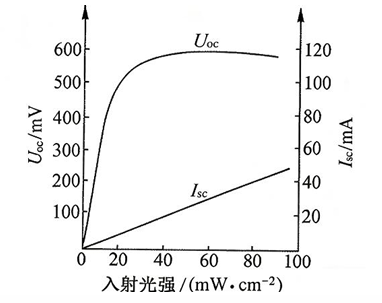
\includegraphics[width=0.5\textwidth]{fig8.png}
     \caption{硅光电池开路电压和短路电路与入射光强的关系曲线}
 \end{figure}

\subsubsection{伏安特性}
在一定光照下，外接不同负载电阻 $R_L$ 时，会有一组 $I, U$ 与之对应，可得伏安特性曲线。
在纵轴上的截距为开路电压 $U_{OC}$，在横轴上的截距为短路电流 $I_{SC}$。

% --- 图9 硅光电池的光照伏安特性 占位 ---
 \begin{figure}[htbp]
     \centering
     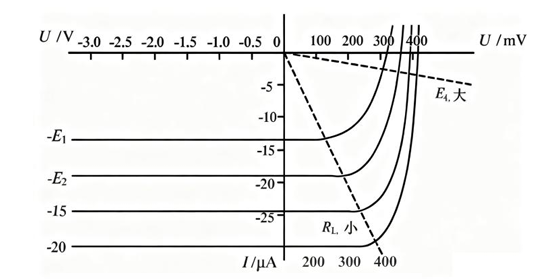
\includegraphics[width=0.5\textwidth]{fig9.png}
     \caption{硅光电池的光照伏安特性}
 \end{figure}

\subsubsection{负载特性与最大输出功率}
当外接负载电阻为 $R_L$ 时，输出电压 $U = I R_L$，输出功率 $P = UI = I^2 R_L$。随着 $R_L$ 增大，输出功率先增大后减小，存在一个最大输出功率 $P_m$，对应此时的负载电阻称为最佳负载电阻 $R_m$。

% --- 图10 某光电池的光照伏安特性曲线(左)及输出功率随负载电阻变化曲线(右) 占位 ---
 \begin{figure}[htbp]
     \centering
     
\includegraphics[width=0.8\textwidth]{fig10.png}
     \caption{左：某光电池的光照伏安特性曲线；右：硅光电池输出功率随负载电阻变化曲线}
 \end{figure}

\subsubsection{填充因子 ($FF$)}
填充因子是衡量硅光电池输出特性优劣的核心指标，定义为最大输出功率与“开路电压 $\times$ 短路电流”的比值：
\begin{equation}
    FF = \frac{P_m}{U_{OC} \cdot I_{SC}}
\end{equation}
$FF$ 越大，则输出功率越高，说明硅光电池对光的利用率越高。

\subsection{光源定标与光强关系}

实验中光源光强无法直接测量，需通过“光源电压 - 光强”定标实现间接换算。由于灯丝温度随电流增加而升高，电阻也会发生很大改变，使得电流电压并非线性关系。实际灯丝电流电压关系为 $U = K \cdot I^n$，转换为 $I = A \cdot U^m$。
做一个近似假设：认为灯泡的光照强度与其实际功率成正比，即：
\begin{equation}
    P_{\text{光强}} = k \cdot P_0 = k \cdot U \cdot I = k \cdot U \cdot A \cdot U^m = B \cdot U^{m+1}
\end{equation}
因此，光强 $P_{\text{光强}}$ 与光源电压 $U_0$ 的关系可通过幂指数拟合得到：$P_{\text{光强}} = B \cdot U_0^{m+1}$，其中 $B$ 为比例系数，$m$ 为与灯丝特性相关的指数。

\section{实验内容}

\subsection{实验一：无光照硅光电池的伏安特性测量}

 \begin{figure}[htbp]
     \centering
     
\includegraphics[width=0.6\textwidth]{fig11.png}
     \caption{无光照时硅光电池的伏安特性测量电路图}
 \end{figure}

\subsubsection{实验操作}
\begin{enumerate}
    \item 将机箱电路图处的盖子打开，电线连接到硅光电池上，盖上盖子；
    \item 取样电阻取 $R = 10\,\Omega$；
    \item 按实验电路图正确接线；
    \item 调节稳压电源 ($0 - 6.0\,\text{V}$)，由于此时硅光电池的特性与二极管特性相同，实验中不宜将电压调至过大，以免烧坏硅光电池，每隔 $0.1\,\text{V}$（视课时而定）记录一组 $U_1$ 与 $U_2$ 的数值；
\end{enumerate}

\textbf{注意：为保证安全，应从小增大电压，另外根据电流变化适当增加取数间隔。}

\subsubsection{数据处理}
\begin{enumerate}
    \item 硅光电池实际电压：$U = U_1 - U_2$（单位：$\text{V}$）；
    \item 通过硅光电池的电流：$I = U_2/10$（单位：$\text{mA}$，因集成板上没有电流表，通过硅光电池的电流需借助取样电阻得到。这里取样电阻为 $10\,\Omega$，由欧姆定律 $I = \frac{U_2}{R_{\text{取样}}}$。此外，取样电阻还具有作为保护电阻对电路进行限流的作用。）
    \item 整理 $U$、$I$ 数据表，绘制 $I - U$ 曲线，用指数函数拟合曲线，对比与普通二极管伏安特性的一致性。
\end{enumerate}

\subsection{实验二：光强不变时，硅光电池的负载特性测量}

 \begin{figure}[htbp]
     \centering
     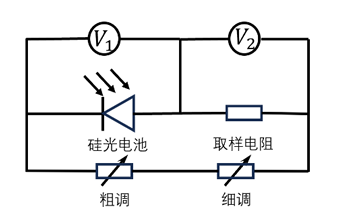
\includegraphics[width=0.6\textwidth]{fig12.png}
     \caption{光强不变时硅光电池的负载特性测量电路图}
 \end{figure}

\subsubsection{实验操作}
\begin{enumerate}
    \item 将机箱电路图处的盖子打开，调整硅光电池面向灯泡照射方向，电线连接到硅光电池上，固定光源与硅光电池距离，盖上盖子；
    \item 按实验电路图正确接线；
    \item 打开光源开关，将光源电压 $U_0$ 调至 $6.0\,\text{V} - 6.5\,\text{V}$ 之间的某一数值（在整个实验过程中，保证光源电压始终不变）；
    \item 调节外接负载，从 $0 - 100\,\text{k}\Omega$，记录硅光电池两端的电压 $U_1$，及取样电阻两端的电压 $U_2$。负载电阻较大时需加密测量，避免错过最大功率点。
\end{enumerate}

\subsubsection{数据处理}
\begin{enumerate}
    \item 根据实验测量数据 $U_1, U_2$，计算硅光电池输出电压 $U = U_1(\text{V})$，和硅光电池输出电流 $I = \frac{U_2}{10}(\text{mA})$；
    \item 计算电池外加负载 $R_L = \frac{U}{I}(\text{k}\Omega)$，输出功率 $P = UI(\text{mW})$；
    \item 整理输出电流 $I$ 与输出电压 $U$ 数据表，及输出功率 $P$ 与外接负载 $R_L$ 的数据表，绘制 $I - U$ 曲线图，及 $P - R_L$ 曲线图。从这些曲线中读取最大输出功率 $P_m$，及对应的 $U_m$、$I_m$、$R_m$；
    \item 读取短路电流 $I_{SC}$（$U=0$ 时的电流）与开路电压 $U_{OC}$（$I=0$ 时的电压）求出硅光电池的填充因子 $FF = \frac{P_m}{I_{SC} \cdot U_{OC}}$。
\end{enumerate}

\subsection{实验三：光源定标（光源电压-光强关系测量）}

 \begin{figure}[htbp]
     \centering
     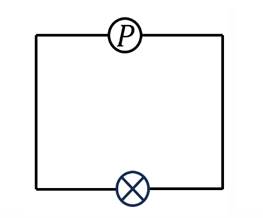
\includegraphics[width=0.6\textwidth]{fig13.png}
     \caption{光源定标测量电路图}
 \end{figure}

\subsubsection{实验操作}
\begin{enumerate}
    \item 将机箱电路图处的盖子打开，调整探测器面向灯泡照射方向，电线连接到探测器上，光源与探测器位置固定，盖上盖子；
    \item 按实验电路图正确接线，将数字电压表换档开关调至“光功率计档”；
    \item 光源电压及功率计进行归零；
    \item 调节光源电压 $U_0$ ($0 - 6.5\,\text{V}$)，每隔 $0.1\,\text{V}$（视课时而定）记录光源电压 $U_0$ 对应光照强度 $P_{\text{光强}}$ 的数值；
\end{enumerate}

\subsubsection{数据处理}
整理 $U_0$、$P_{\text{光强}}$ 数据表，以 $U_0$ 为横坐标、$P_{\text{光强}}$ 为纵坐标绘制曲线，并进行幂指数函数拟合，得到 $P_{\text{光强}} = B \cdot U_0^{m+1}$ 的经验公式，以便用于后续光强换算。

\subsection{实验四：开路电压 $U_{OC}$ 与相对光强的关系测量}

 \begin{figure}[htbp]
     \centering
     
\includegraphics[width=0.6\textwidth]{fig14.png}
     \caption{开路电压与相对光强关系测量的电路图}
 \end{figure}

\subsubsection{实验操作}
\begin{enumerate}
    \item 将机箱电路图处的盖子打开，调整硅光电池面向灯泡照射方向；
    \item 按实验电路图正确接线，将硅光电池输出端开路（不接负载）。注意电压表连接大量程的电压表 ($0 - 20\,\text{V}$)；
    \item 调节光源电压 $U_0$ ($0 - 6.5\,\text{V}$)，每隔 $0.1\,\text{V}$（视课时而定）记录对应开路电压 $U_{OC}$ 的数值；
\end{enumerate}

\subsubsection{数据处理}
\begin{enumerate}
    \item 依据预实验的定标得到的经验公式 $P_{\text{光强}} = B \cdot U_0^{m+1}$，将光源电压 $U_0$ 的数值转换为光照强度 $P_{\text{光强}}$，定义某一光强为基准 $P_0$，计算相对光强 $\frac{P_i}{P_0}$；
    \item 整理 $\frac{P_i}{P_0}$、$U_{OC}$ 数据表，绘制 $U_{OC} - \ln\left(\frac{P_i}{P_0}\right)$ 曲线，用对数函数拟合，验证 $U_{OC}$ 随相对光强对数增长的规律：
    \[ U_{OC} = \frac{nkT}{e} \cdot \ln \left( \frac{I_{ph}}{I_0} + 1 \right) \approx \frac{nkT}{e} \cdot \ln \left( \frac{I_{ph}}{I_0} \right) \approx K \cdot \ln \left( \frac{P_i}{P_0} \right) \]
\end{enumerate}

\subsection{实验五：短路电流 $I_{SC}$ 与相对光强的关系测量}

 \begin{figure}[htbp]
     \centering
     
\includegraphics[width=0.6\textwidth]{fig15.png}
     \caption{短路电流与相对光强关系测量的电路图}
 \end{figure}

\subsubsection{实验操作}
\begin{enumerate}
    \item 取样电阻取 $R_{\text{取样}} = 10\,\Omega$（直接小取样电阻即外接极小负载，近似短路）；数字电压表测量取样电阻两端电压 $U_2$（注意连接 $m\text{V}$ 量程的电压表）；
    \item 光源电压 $U_0$ 从 $0\,\text{V}$ 逐步调节至 $6.5\,\text{V}$，每隔 $0.5\,\text{V}$ 记录一组 $U_0$ 与 $U_2$ 的数据（因低电压时 $I_{SC}$ 过小，测量误差较大，此时应增大电压间隔）；
\end{enumerate}

\subsubsection{数据处理}
\begin{enumerate}
    \item 依据实验三定标得到的经验公式 $P_{\text{光强}} = B \cdot U_0^{m+1}$，将光源电压 $U_0$ 的数值转换为光照强度 $P_{\text{光强}}$，定义某一光强为基准 $P_0$，计算相对光强 $\frac{P_i}{P_0}$；
    \item 依据本实验测量的取样电阻两端电压 $U_2$，计算短路电流 $I_{SC} = \frac{U_2}{10}(\text{mA})$；
    \item 整理 $\frac{P_i}{P_0}$、$I_{SC}$ 数据表，绘制 $I_{SC} - \frac{P_i}{P_0}$ 曲线，用线性函数拟合，验证 $I_{SC}$ 随相对光强线性增长的规律。
\end{enumerate}

\subsection{实验六：反向偏压状态下硅光电池的光电特性}

 \begin{figure}[htbp]
     \centering
     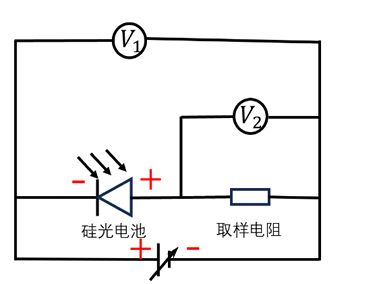
\includegraphics[width=0.6\textwidth]{fig16.png}
     \caption{反向偏置下电流与相对光强关系的电路图}
 \end{figure}

\subsubsection{实验操作}
\begin{enumerate}
    \item 连接电路，电路与实验一电路相似，但稳压电源接入极性相反；
    \item 取样电阻取 $R_{\text{取样}} = 10\,\Omega$；
    \item 设置光源电压 $U_0$ 分别为 $2\,\text{V}$、$3\,\text{V}$ 和 $4\,\text{V}$ 时，调节电源电压 $U_1$，从 $0\,\text{V}$ 逐步调节至 $6.5\,\text{V}$，每隔 $0.5\,\text{V}$ 记录取样电阻两端的电压 $U_2$ 数据；
\end{enumerate}

\subsubsection{数据处理}
\begin{enumerate}
    \item 依据本实验测量的取样电阻两端电压 $U_2$，计算通过硅光电池的电流 $I = \frac{U_2}{10}(\text{mA})$；
    \item 计算硅光电池两端的电压 $U = U_1 - U_2$；
    \item 整理 $U$、$I$ 数据表，绘制 $I - U$ 曲线，将不同 $U_0$ 下的 $I - U$ 曲线画到一个图里。
\end{enumerate}

\section{实验数据}
\subsection{无光照下，硅光电池的伏安特性（计算硅光电池两端电压及通过电流，绘制 $I-U$ 曲线）}

取样电阻 $R_{\text{取样}} = 10\,\Omega$

\begin{table}[htbp]
    \centering
    \caption{无光照下硅光电池伏安特性原始数据记录表}
    \label{tab:dark_raw}
    \begin{tabular}{cc|cc|cc}
        \toprule
        $U_1 / \text{V}$ & $U_2 / \text{mV}$ & $U_1 / \text{V}$ & $U_2 / \text{mV}$ & $U_1 / \text{V}$ & $U_2 / \text{mV}$ \\
        \midrule
        1.26 & 0.00 & 2.96 & 1.2  & 4.66 & 14.4  \\
        1.36 & 0.1  & 3.06 & 1.3  & 4.76 & 16.9  \\
        1.46 & 0.1  & 3.16 & 1.6  & 4.86 & 20.1  \\
        1.56 & 0.1  & 3.26 & 1.8  & 4.96 & 23.9  \\
        1.66 & 0.1  & 3.36 & 2.1  & 5.06 & 28.7  \\
        1.76 & 0.2  & 3.46 & 2.4  & 5.16 & 35.4  \\
        1.86 & 0.2  & 3.56 & 2.7  & 5.26 & 42.7  \\
        1.96 & 0.3  & 3.66 & 3.1  & 5.36 & 52.8  \\
        2.06 & 0.3  & 3.76 & 3.6  & 5.46 & 64.9  \\
        2.16 & 0.4  & 3.86 & 4.2  & 5.56 & 78.9  \\
        2.26 & 0.4  & 3.96 & 4.9  & 5.66 & 95.1  \\
        2.36 & 0.5  & 4.06 & 5.7  & 5.76 & 114.9 \\
        2.46 & 0.6  & 4.16 & 6.6  & 5.86 & 138.6 \\
        2.56 & 0.7  & 4.26 & 7.6  & 5.96 & 166.5 \\
        2.66 & 0.8  & 4.36 & 8.9  & 6.00 & 176.4 \\
        2.76 & 0.9  & 4.46 & 10.4 &      &       \\
        2.86 & 1.0  & 4.56 & 12.2 &      &       \\
        \bottomrule
    \end{tabular}
\end{table}

\textbf{数据处理：}
\begin{enumerate}
    \item[(1)] 硅光电池两端实际电压：$U = U_1 - U_2$（单位：$\text{V}$）；
    \item[(2)] 通过硅光电池的电流：$I = U_2/10$（单位：$\text{mA}$，因集成板上没有电流表，通过硅光电池的电流需借助取样电阻得到。这里取样电阻为 $10\,\Omega$，由欧姆定律 $I = \frac{U_2}{R_{\text{取样}}}$；
    \item[(3)] 整理 $U$、$I$ 数据表，绘制 $I-U$ 曲线，用指数函数拟合曲线，对比与普通二极管伏安特性的一致性。
\end{enumerate}

\textbf{数据处理结果：}

根据原始数据\cref{tab:dark_raw}，计算得到的硅光电池两端电压 $U = U_1 - U_2/1000$ (V) 和通过电流 $I = U_2/10$ (mA)，如\cref{tab:dark_processed}所示。

\begin{table}[htbp]
    \centering
    \caption{无光照下硅光电池伏安特性处理数据表}
    \label{tab:dark_processed}
    \begin{tabular}{cc|cc|cc}
        \toprule
        $U / \text{V}$ & $I / \text{mA}$ & $U / \text{V}$ & $I / \text{mA}$ & $U / \text{V}$ & $I / \text{mA}$ \\
        \midrule
        1.26 & 0.00 & 2.96 & 0.12 & 4.65 & 1.44 \\
        1.36 & 0.01 & 3.06 & 0.13 & 4.74 & 1.69 \\
        1.46 & 0.01 & 3.16 & 0.16 & 4.84 & 2.01 \\
        1.56 & 0.01 & 3.26 & 0.18 & 4.94 & 2.39 \\
        1.66 & 0.01 & 3.36 & 0.21 & 5.03 & 2.87 \\
        1.76 & 0.02 & 3.46 & 0.24 & 5.12 & 3.54 \\
        1.86 & 0.02 & 3.56 & 0.27 & 5.22 & 4.27 \\
        1.96 & 0.03 & 3.66 & 0.31 & 5.31 & 5.28 \\
        2.06 & 0.03 & 3.76 & 0.36 & 5.40 & 6.49 \\
        2.16 & 0.04 & 3.86 & 0.42 & 5.48 & 7.89 \\
        2.26 & 0.04 & 3.96 & 0.49 & 5.56 & 9.51 \\
        2.36 & 0.05 & 4.05 & 0.57 & 5.65 & 11.49 \\
        2.46 & 0.06 & 4.15 & 0.66 & 5.72 & 13.86 \\
        2.56 & 0.07 & 4.25 & 0.76 & 5.79 & 16.65 \\
        2.66 & 0.08 & 4.35 & 0.89 & 5.82 & 17.64 \\
        2.76 & 0.09 & 4.45 & 1.04 &  &  \\
        2.86 & 0.10 & 4.55 & 1.22 &  &  \\
        \bottomrule
    \end{tabular}
\end{table}

绘制 $I-U$ 曲线并进行指数函数拟合，结果如\cref{fig:dark_iu}所示。

\begin{figure}[htbp]
    \centering
    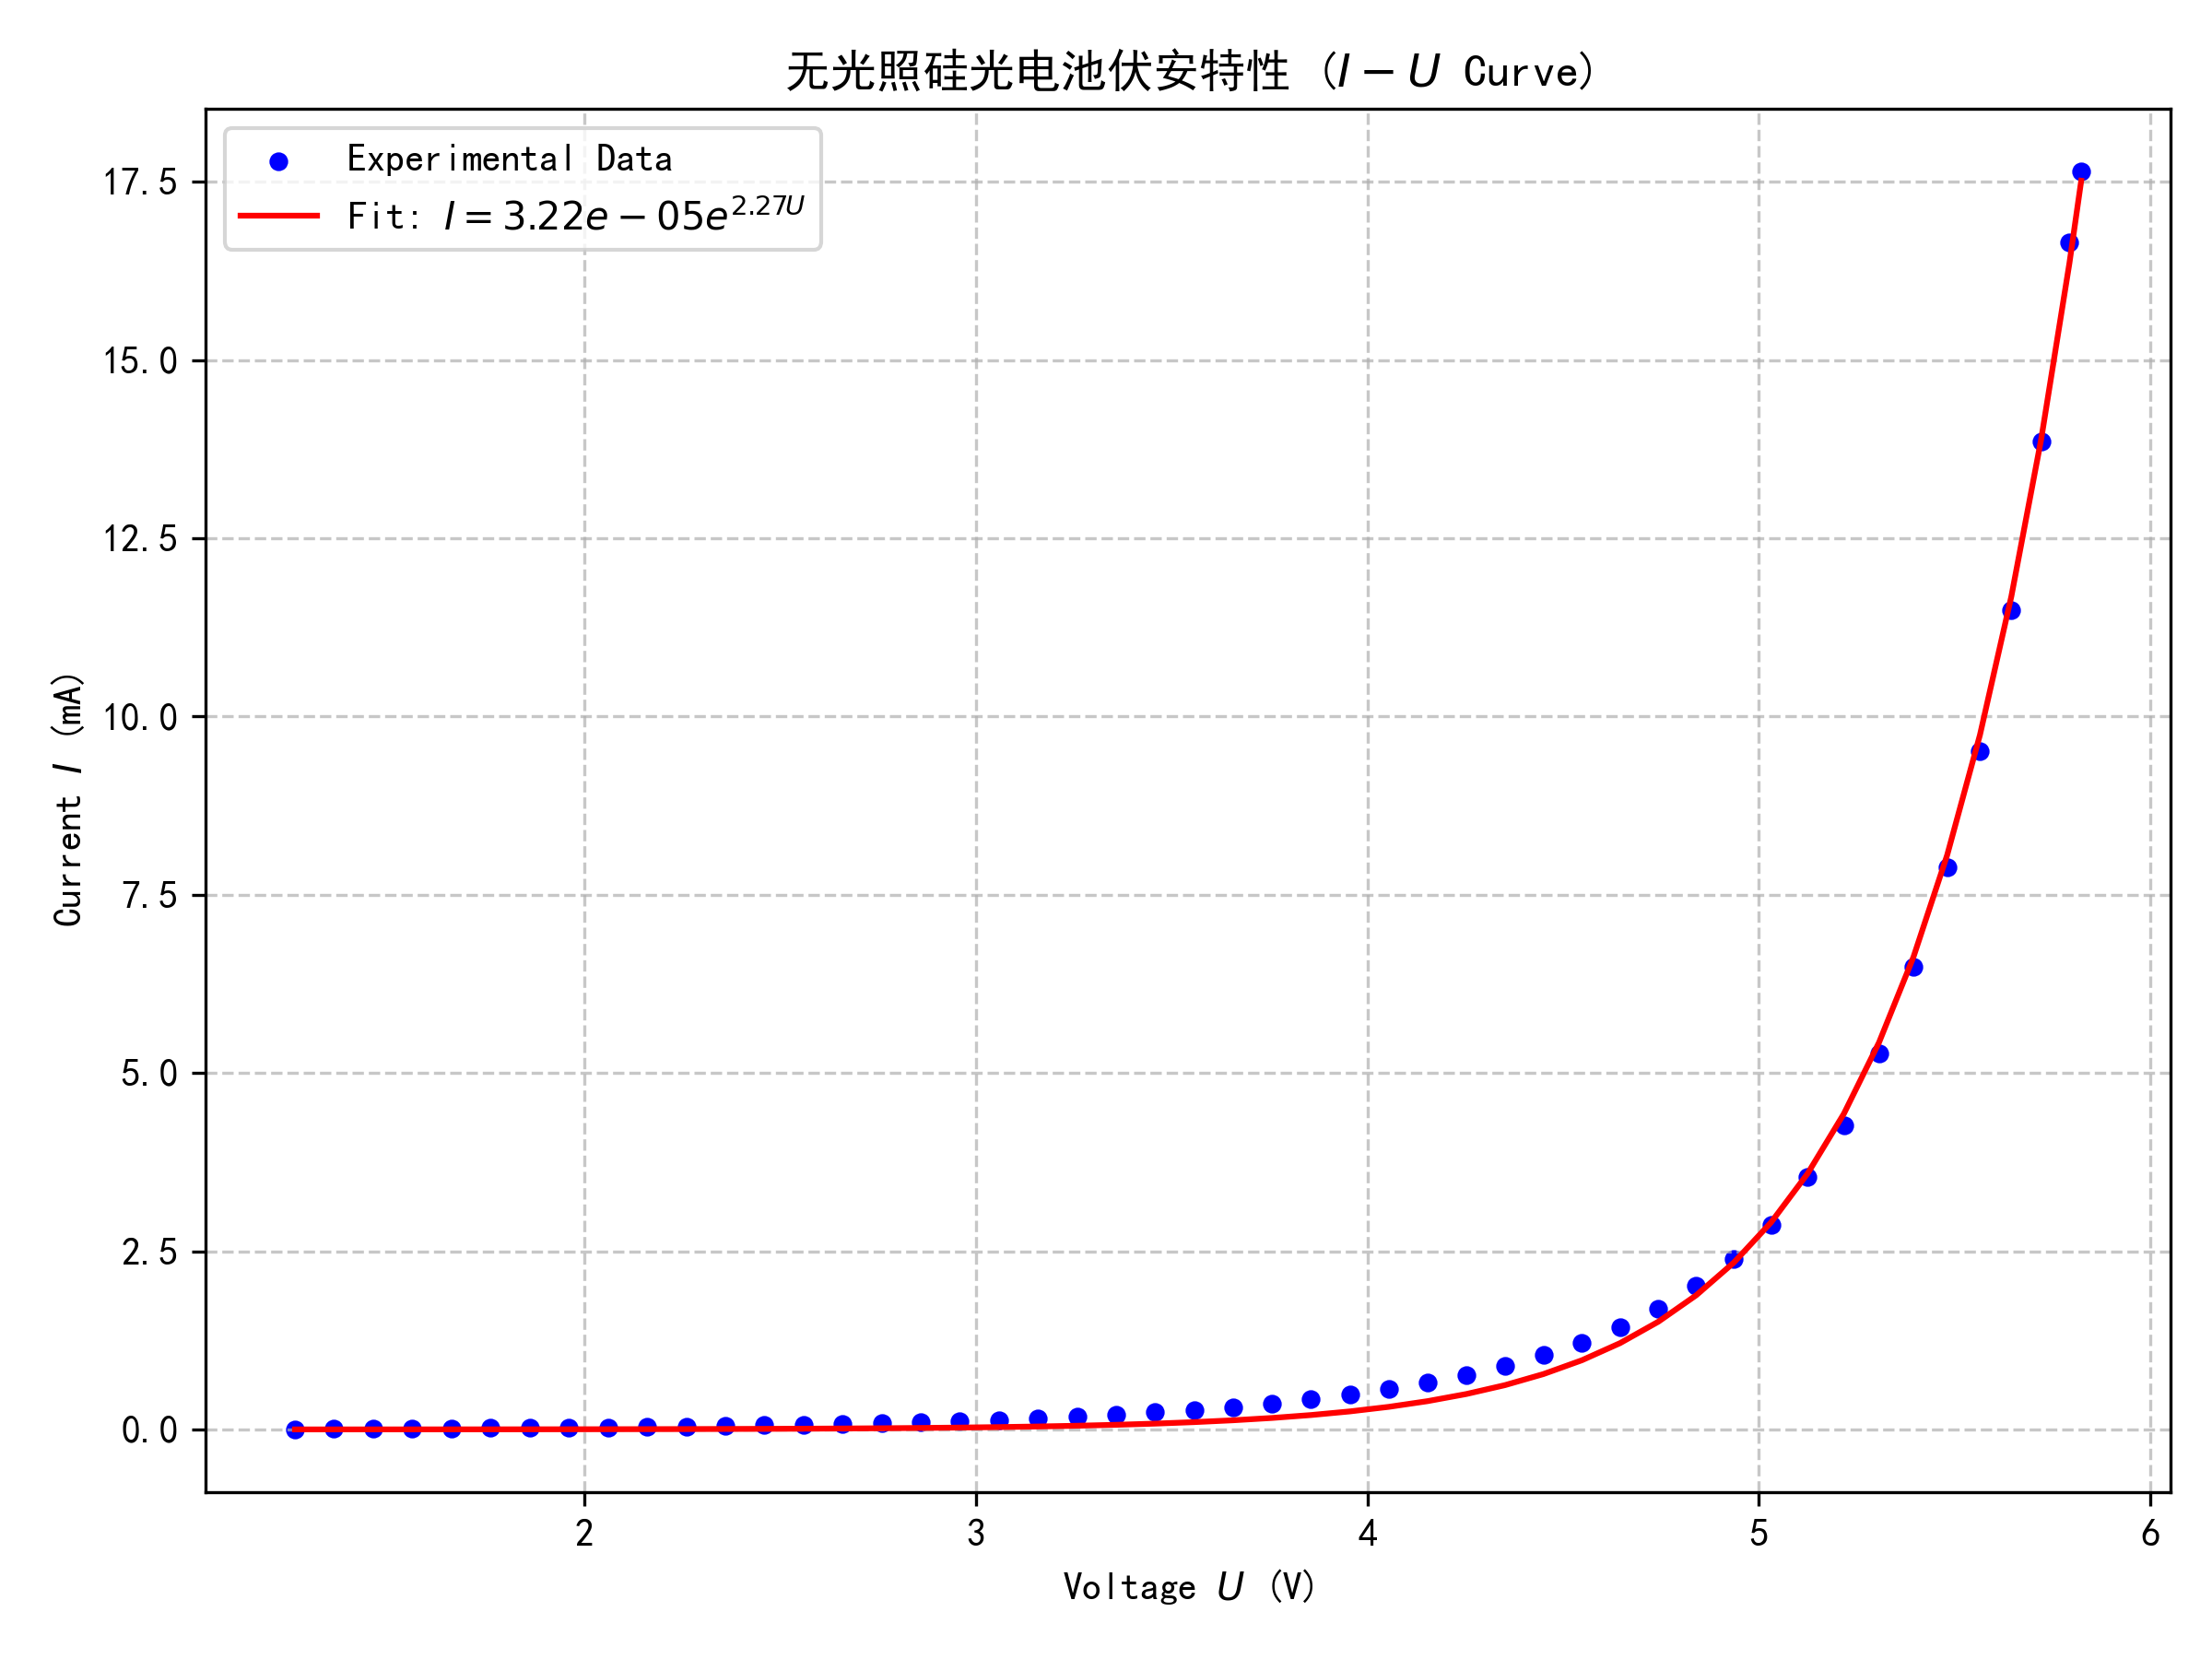
\includegraphics[width=0.7\textwidth]{fig_experiment1.png}
    \caption{无光照下硅光电池伏安特性曲线及拟合}
    \label{fig:dark_iu}
\end{figure}

拟合公式为：$I = 3.22 \times 10^{-5} \cdot e^{2.27 U}$。
可见，在无光照条件下，硅光电池的伏安特性曲线呈指数增长关系，符合二极管的正向导通特性。

\subsection{光强不变，硅光电池的负载特性（绘制 $I-U$ 曲线图，及 $P-R_L$ 曲线图；得到 $P_m$、$U_m$、$I_m$、$R_m$ 数值；计算 $FF$ 值）}

光源电压 $U_0 = 6.19\,\text{V}$，取样电阻 $R_{\text{取样}} = 10\,\Omega$

\begin{table}[htbp]
    \centering
    \caption{硅光电池负载特性原始数据记录表}
    \label{tab:load_raw}
    \begin{tabular}{cc|cc|cc}
        \toprule
        $U_1 / \text{V}$ & $U_2 / \text{mV}$ & $U_1 / \text{V}$ & $U_2 / \text{mV}$ & $U_1 / \text{V}$ & $U_2 / \text{mV}$ \\
        \midrule
        0.0 & 7.7 & 2.2 & 6.7 & 4.05 & 6.3 \\
        0.2 & 7.6 & 2.4 & 6.7 & 4.1  & 6.2 \\
        0.4 & 7.5 & 2.6 & 6.6 & 4.15 & 6.2 \\
        0.6 & 7.4 & 2.8 & 6.5 & 4.2  & 6.2 \\
        0.8 & 7.3 & 3.0 & 6.5 & 4.22 & 6.0 \\
        1.0 & 7.2 & 3.4 & 6.4 & 4.25 & 5.9 \\
        1.2 & 7.1 & 3.8 & 6.3 & 4.4  & 5.2 \\
        1.4 & 7.0 & 3.94 & 6.3 & 4.6  & 2.1 \\
        1.6 & 6.9 & 4.0 & 6.3 & 4.65 & 0.4 \\
        1.8 & 6.8 & 2.0 & 6.8 & & \\
        \bottomrule
    \end{tabular}
\end{table}

\textbf{数据处理：}
\begin{enumerate}
    \item[(1)] 根据实验测量数据 $U_1, U_2$，计算硅光电池输出电压 $U = U_1(\text{V})$，和硅光电池输出电流 $I = \frac{U_2}{10}(\text{mA})$；
    \item[(2)] 计算电池外加负载 $R_L = \frac{U}{I}(\text{k}\Omega)$，输出功率 $P = UI(\text{mW})$；
    \item[(3)] 整理输出电流 $I$ 与输出电压 $U$ 数据表，及输出功率 $P$ 与外接负载 $R_L$ 的数据表，绘制 $I-U$ 曲线图，及 $P-R_L$ 曲线图。从这些曲线中读取最大输出功率 $P_m$，及对应的 $U_m$、$I_m$、$R_m$；
    \item[(4)] 读取短路电流 $I_{SC}$（$U=0$ 时的电流）与开路电压 $U_{OC}$（$I=0$ 时的电压）求出硅光电池的填充因子 $FF = \frac{P_m}{I_{SC} \cdot U_{OC}}$。
\end{enumerate}

\textbf{数据处理结果：}

根据原始数据\cref{tab:load_raw}，计算得到的硅光电池两端电压 $U$、输出电流 $I$、负载电阻 $R_L$ 及输出功率 $P$ 如\cref{tab:load_processed}所示。

\begin{table}[htbp]
    \centering
    \caption{硅光电池负载特性处理数据表}
    \label{tab:load_processed}
    \resizebox{\textwidth}{!}{
    \begin{tabular}{cccc|cccc}
        \toprule
        $U / \text{V}$ & $I / \text{mA}$ & $R_L / \text{k}\Omega$ & $P / \text{mW}$ & $U / \text{V}$ & $I / \text{mA}$ & $R_L / \text{k}\Omega$ & $P / \text{mW}$ \\
        \midrule
        0.00 & 0.77 & 0.00 & 0.00 & 3.00 & 0.65 & 4.62 & 1.95 \\
        0.20 & 0.76 & 0.26 & 0.15 & 3.40 & 0.64 & 5.31 & 2.18 \\
        0.40 & 0.75 & 0.53 & 0.30 & 3.80 & 0.63 & 6.03 & 2.39 \\
        0.60 & 0.74 & 0.81 & 0.44 & 3.94 & 0.63 & 6.25 & 2.48 \\
        0.80 & 0.73 & 1.10 & 0.58 & 4.00 & 0.63 & 6.35 & 2.52 \\
        1.00 & 0.72 & 1.39 & 0.72 & 4.05 & 0.63 & 6.43 & 2.55 \\
        1.20 & 0.71 & 1.69 & 0.85 & 4.10 & 0.62 & 6.61 & 2.54 \\
        1.40 & 0.70 & 2.00 & 0.98 & 4.15 & 0.62 & 6.69 & 2.57 \\
        1.60 & 0.69 & 2.32 & 1.10 & 4.20 & 0.62 & 6.77 & 2.60 \\
        1.80 & 0.68 & 2.65 & 1.22 & 4.22 & 0.60 & 7.03 & 2.53 \\
        2.00 & 0.68 & 2.94 & 1.36 & 4.25 & 0.59 & 7.20 & 2.51 \\
        2.20 & 0.67 & 3.28 & 1.47 & 4.40 & 0.52 & 8.46 & 2.29 \\
        2.40 & 0.67 & 3.58 & 1.61 & 4.60 & 0.21 & 21.90 & 0.97 \\
        2.60 & 0.66 & 3.94 & 1.72 & 4.65 & 0.04 & 116.25 & 0.19 \\
        2.80 & 0.65 & 4.31 & 1.82 & & & & \\
        \bottomrule
    \end{tabular}}
\end{table}

绘制 $I-U$ 曲线及 $P-U$ 曲线、 $P-R_L$ 曲线如\cref{fig:load_iu_pu}、\cref{fig:load_p_rl}所示。

\begin{figure}[htbp]
    \centering
    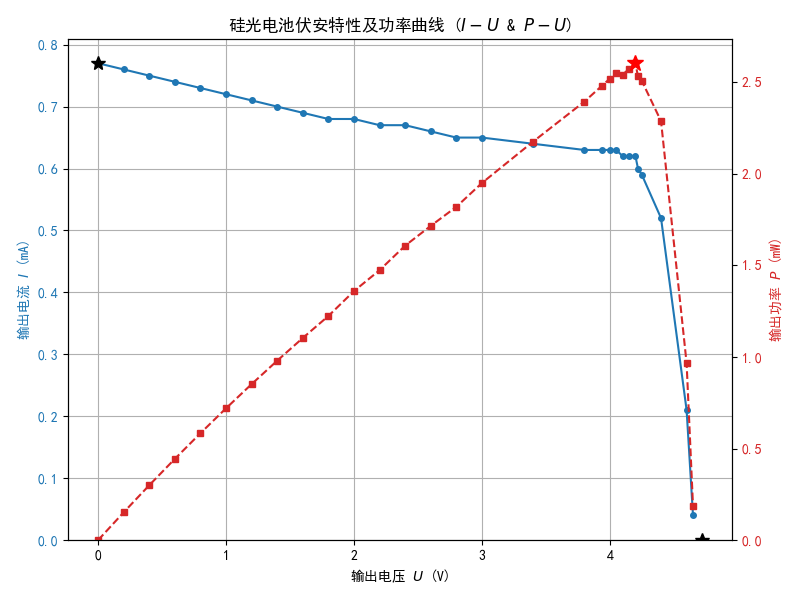
\includegraphics[width=0.7\textwidth]{fig_experiment2_IU_PU.png}
    \caption{硅光电池伏安特性及功率曲线}
    \label{fig:load_iu_pu}
\end{figure}

\begin{figure}[htbp]
    \centering
    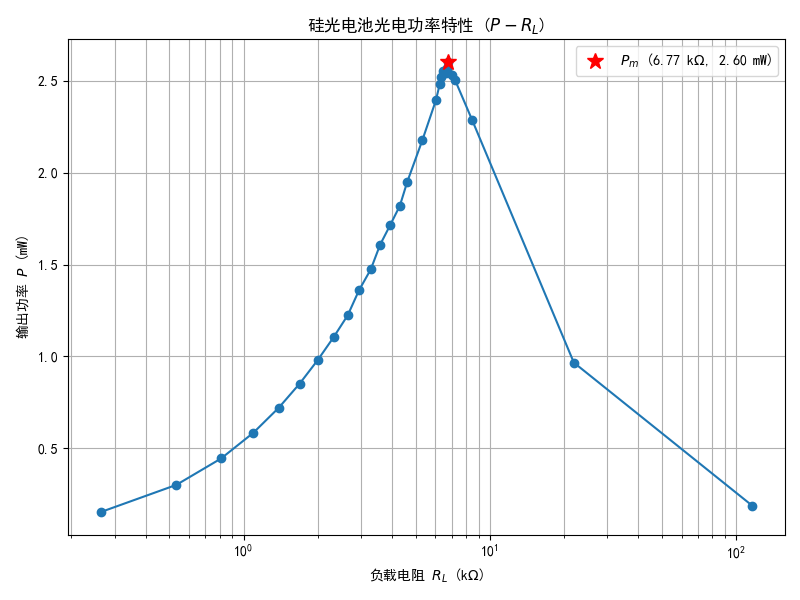
\includegraphics[width=0.7\textwidth]{fig_experiment2_P_RL.png}
    \caption{硅光电池输出功率随负载电阻变化曲线}
    \label{fig:load_p_rl}
\end{figure}

从数据表和曲线中读取并计算得到：
\begin{enumerate}
    \item 最大输出功率 $P_m = 2.60\,\text{mW}$，对应的电压 $U_m = 4.20\,\text{V}$，电流 $I_m = 0.62\,\text{mA}$，最佳负载电阻 $R_m = 6.77\,\text{k}\Omega$。
    \item 短路电流 $I_{SC} = 0.77\,\text{mA}$。
    \item 通过线性外推得到的开路电压 $U_{OC} \approx 4.72\,\text{V}$。
    \item 填充因子 $FF = \frac{P_m}{I_{SC} \cdot U_{OC}} = \frac{2.60}{0.77 \times 4.72} \approx 0.72$。
\end{enumerate}

\subsection{光源定标（绘制 $P_{\text{光强}} - U_0$ 曲线，得到 $P_{\text{光强}}$ 经验公式）}


\begin{table}[htbp]
    \centering
    \caption{光源定标原始数据记录汇总表}
    \label{tab:calibration_raw}
    \begin{tabular}{cc|cc|cc}
        \toprule
        $U_0 / \text{V}$ & $P_{\text{光强}} / \text{mW}$ & $U_0 / \text{V}$ & $P_{\text{光强}} / \text{mW}$ & $U_0 / \text{V}$ & $P_{\text{光强}} / \text{mW}$ \\
        \midrule
        0    & 0   & 2.64 & 4.6  & 4.18 & 28.2 \\
        1.22 & 0.1 & 2.75 & 5.5  & 4.28 & 31.2 \\
        1.34 & 0.1 & 2.86 & 6.4  & 4.40 & 34.2 \\
        1.43 & 0.2 & 2.96 & 7.5  & 4.48 & 36.2 \\
        1.56 & 0.3 & 3.07 & 8.8  & 4.59 & 39.1 \\
        1.66 & 0.4 & 3.15 & 9.6  & 4.69 & 41.8 \\
        1.76 & 0.6 & 3.26 & 11.1 & 4.79 & 44.6 \\
        1.86 & 0.8 & 3.37 & 12.8 & 4.89 & 47.3 \\
        1.96 & 1.1 & 3.47 & 14.4 & 4.99 & 49.8 \\
        2.06 & 1.4 & 3.60 & 16.5 & 5.07 & 52.0 \\
        2.15 & 1.7 & 3.68 & 17.7 & 5.17 & 54.5 \\
        2.26 & 2.2 & 3.79 & 20.1 & 5.31 & 58.3 \\
        2.36 & 2.8 & 3.89 & 22.4 & 5.37 & 59.3 \\
        2.46 & 3.3 & 3.98 & 24.2 & 5.46 & 62.0 \\
        2.55 & 3.8 & 4.08 & 26.3 & 5.58 & 64.6 \\
        5.69 & 67.5 & 5.99 & 74.7 & 6.25 & 80.6 \\
        5.79 & 69.9 & 6.07 & 76.4 & 6.42 & 84.7 \\
        5.89 & 73.2 & 6.19 & 79.2 & 6.53 & 87.5 \\
        \bottomrule
    \end{tabular}
\end{table}

\textbf{数据处理：}
整理 $U_0$、$P_{\text{光强}}$ 数据表，绘制 $P_{\text{光强}} - U_0$ 曲线，并进行幂指数函数拟合，得到 $P_{\text{光强}} = B \cdot U_0^{m+1}$ 的经验公式，以便用于后续光强换算。

\textbf{数据处理结果：}

根据\cref{tab:calibration_raw}中的原始数据，绘制 $P_{\text{光强}} - U_0$ 曲线并进行幂指数函数拟合，结果如\cref{fig:calibration}所示。

\begin{figure}[htbp]
    \centering
    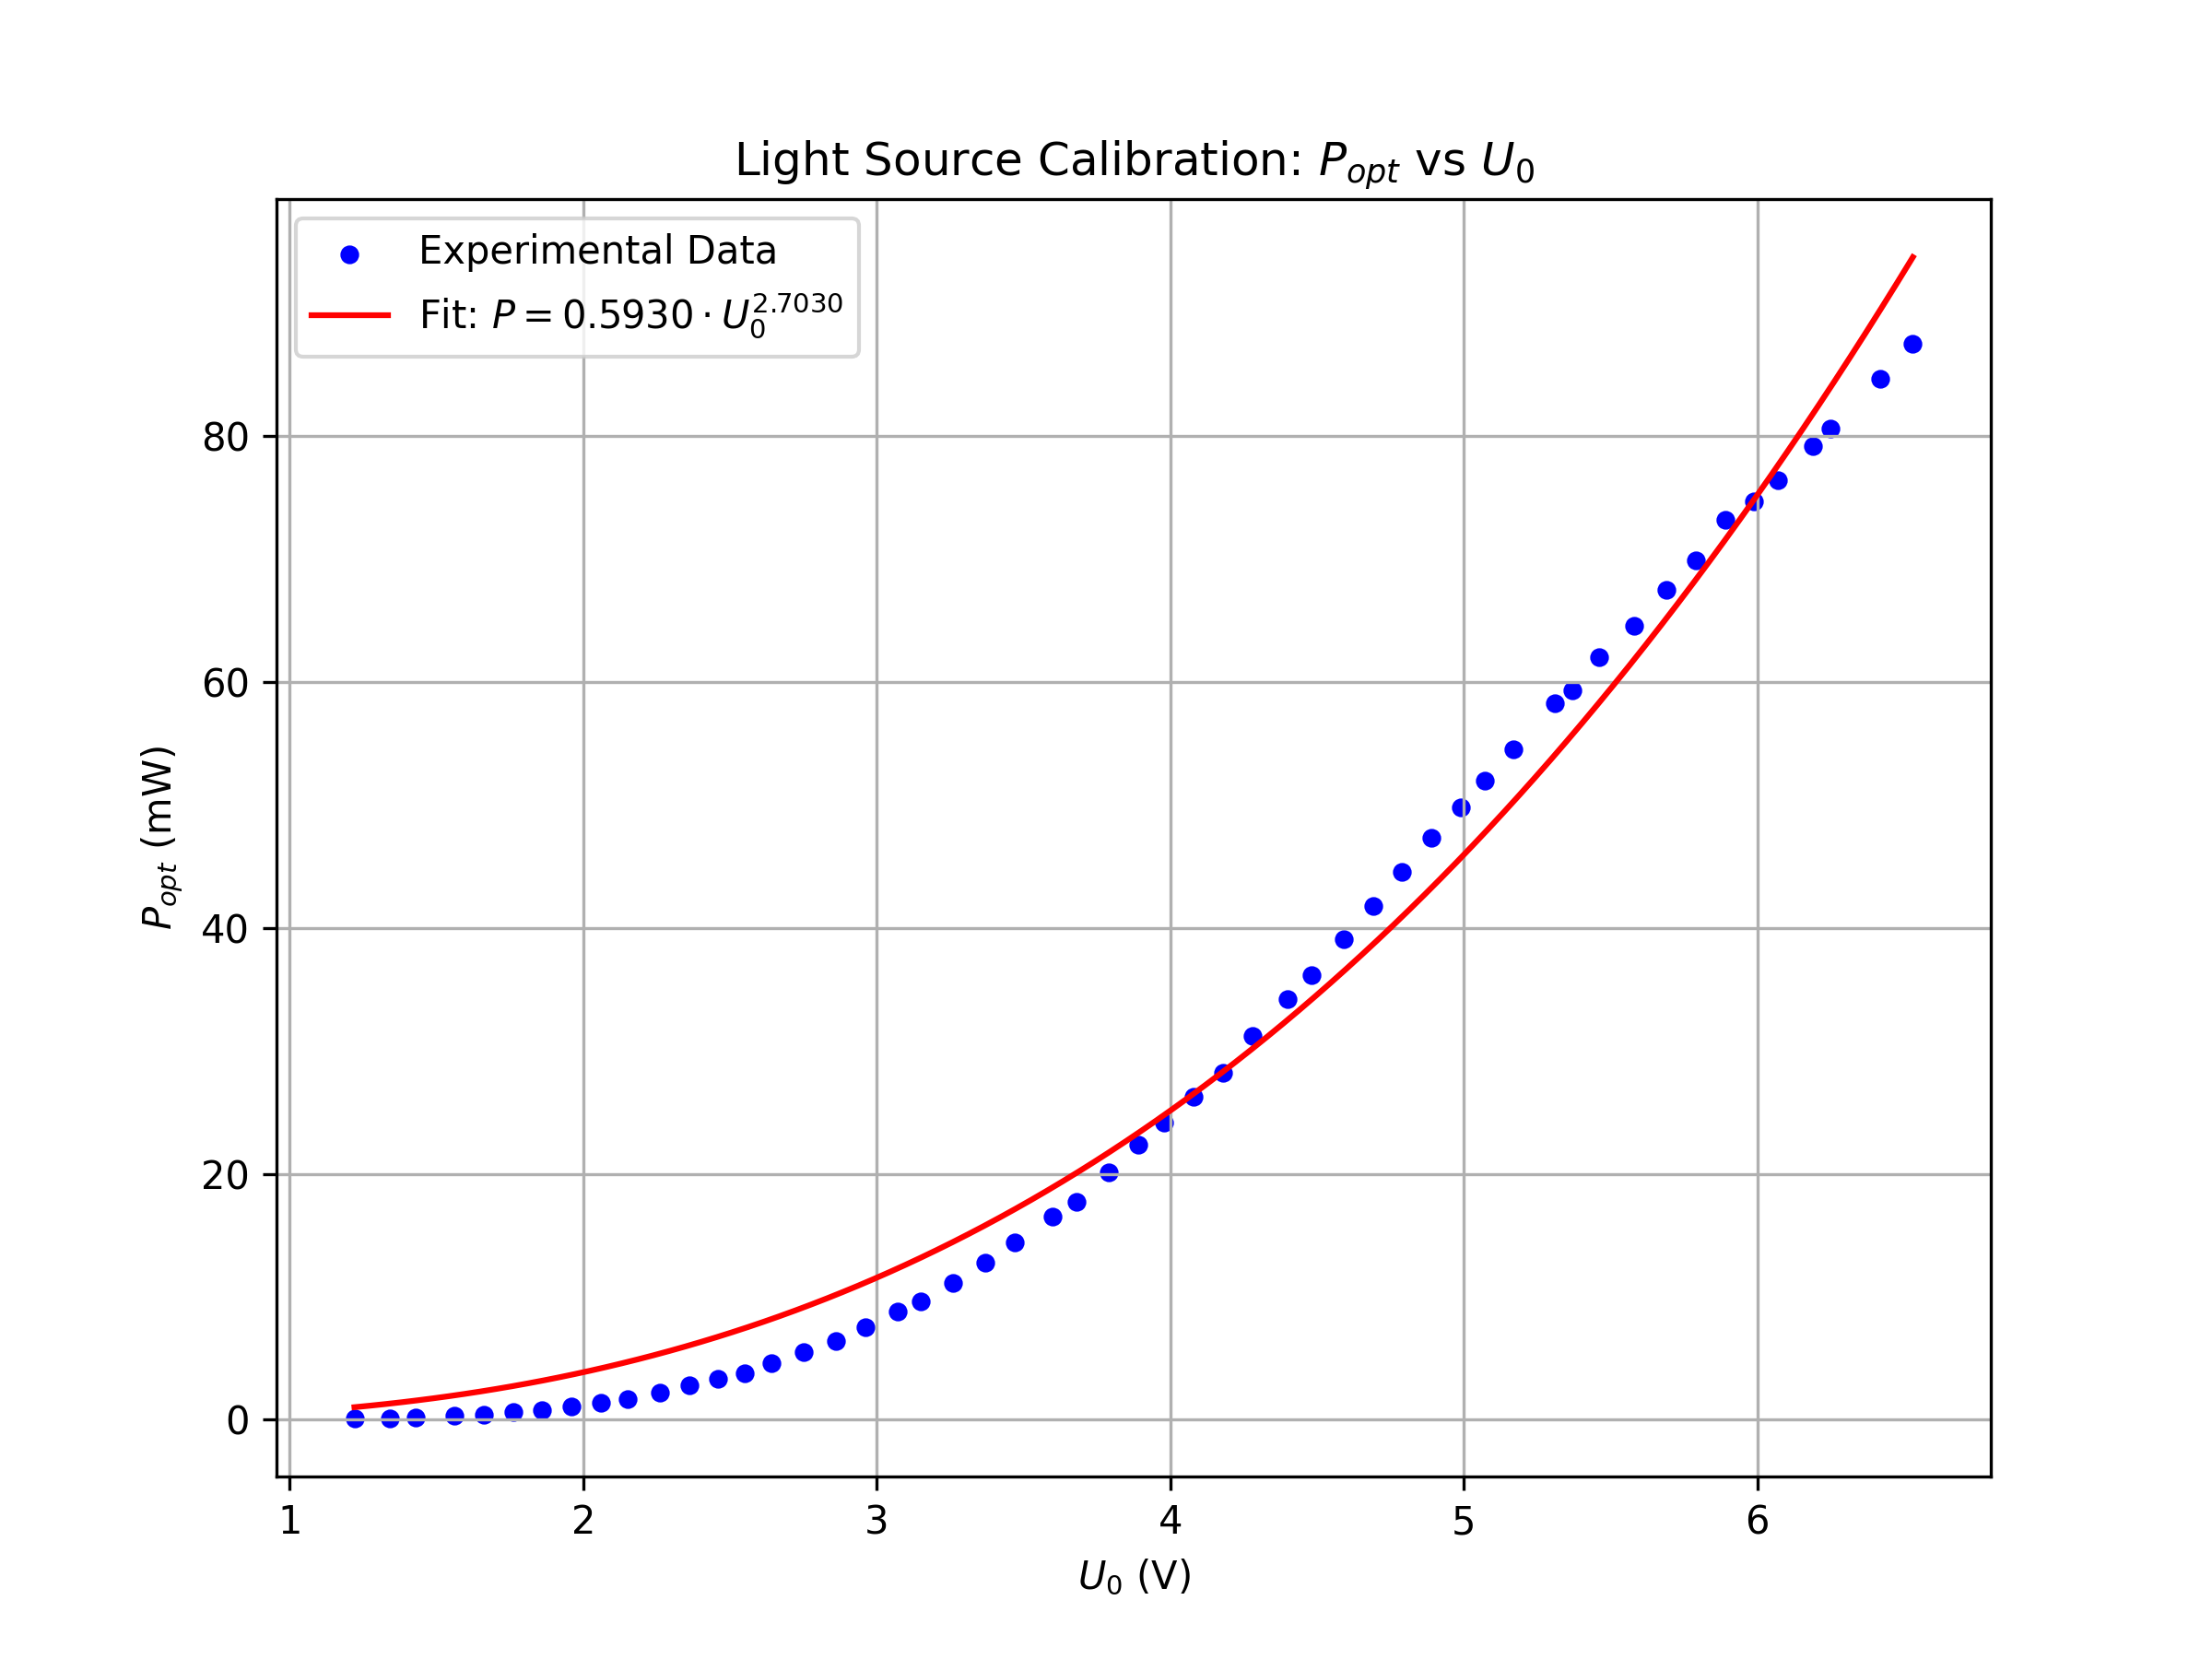
\includegraphics[width=0.7\textwidth]{fig_experiment3.png}
    \caption{光源定标曲线及拟合}
    \label{fig:calibration}
\end{figure}

拟合得到的经验公式为：
\begin{equation}
    P_{\text{光强}} = 0.5930 \cdot U_0^{2.7030}
\end{equation}
其中系数 $B = 0.5930$，指数项 $m+1 = 2.7030$。该经验公式将用于后续实验中的光强换算。

\subsection{开路电压 $U_{OC}$ 与相对光强的关系}


\begin{table}[htbp]
    \centering
    \caption{开路电压测量原始数据记录表}
    \label{tab:exp4_raw}
    \begin{tabular}{cc|cc|cc}
        \toprule
        $U_0 / \text{V}$ & $U_{OC} / \text{V}$ & $U_0 / \text{V}$ & $U_{OC} / \text{V}$ & $U_0 / \text{V}$ & $U_{OC} / \text{V}$ \\
        \midrule
        0    & 0.01 & 2.50 & 2.32 & 4.39 & 3.95 \\
        0.76 & 0.01 & 2.59 & 2.44 & 4.50 & 4.01 \\
        0.87 & 0.02 & 2.69 & 2.56 & 4.60 & 4.06 \\
        0.99 & 0.05 & 2.81 & 2.71 & 4.70 & 4.11 \\
        1.10 & 0.11 & 2.88 & 2.79 & 4.80 & 4.15 \\
        1.20 & 0.20 & 2.98 & 2.89 & 4.94 & 4.22 \\
        1.29 & 0.32 & 3.09 & 3.00 & 5.04 & 4.26 \\
        1.38 & 0.46 & 3.19 & 3.10 & 5.16 & 4.31 \\
        1.49 & 0.63 & 3.29 & 3.18 & 5.27 & 4.35 \\
        1.59 & 0.83 & 3.37 & 3.26 & 5.37 & 4.38 \\
        1.68 & 0.98 & 3.49 & 3.36 & 5.46 & 4.41 \\
        1.77 & 1.15 & 3.60 & 3.44 & 5.57 & 4.45 \\
        1.86 & 1.33 & 3.69 & 3.50 & 5.70 & 4.49 \\
        2.01 & 1.58 & 3.80 & 3.59 & 5.82 & 4.52 \\
        2.13 & 1.77 & 3.90 & 3.66 & 5.90 & 4.54 \\
        2.20 & 1.89 & 4.08 & 3.77 & 6.00 & 4.57 \\
        2.30 & 2.05 & 4.20 & 3.84 & 6.10 & 4.60 \\
        2.41 & 2.19 & 4.38 & 3.88 & 6.24 & 4.63 \\
             &      &      &      & 6.32 & 4.65 \\
             &      &      &      & 6.47 & 4.68 \\
        \bottomrule
    \end{tabular}
\end{table}

\textbf{数据处理：}
\begin{enumerate}
    \item[(1)] 依据实验三的定标，将光源电压 $U_0$ 的数值转换为光照强度 $P_{\text{光强}}$，定义某一光强为基准 $P_0$，计算相对光强 $\frac{P_i}{P_0}$；
    \item[(2)] 整理 $\frac{P_i}{P_0}$、$U_{OC}$ 数据表，绘制 $U_{OC} - \ln\left(\frac{P_i}{P_0}\right)$ 曲线，用对数函数拟合，验证 $U_{OC}$ 随相对光强对数增长的规律：
    \[ U_{OC} = \frac{nkT}{e} \cdot \ln\left(\frac{I_{ph}}{I_0} + 1\right) \approx \frac{nkT}{e} \cdot \ln\left(\frac{I_{ph}}{I_0}\right) \approx K \cdot \ln\left(\frac{P_i}{P_0}\right) \]
\end{enumerate}
\textbf{数据处理结果：}

根据\cref{tab:exp4_raw}中的原始数据，结合实验三得到的经验公式 $P_{\text{光强}} = 0.5930 \cdot U_0^{2.7030}$ 计算光照强度，并以最大光强 $P_0$ 为基准计算相对光强。以 $\ln(P_i/P_0)$ 为横坐标，$U_{OC}$ 为纵坐标绘制曲线，如图\ref{fig:uoc_lnp}所示。

\begin{figure}[htbp]
    \centering
    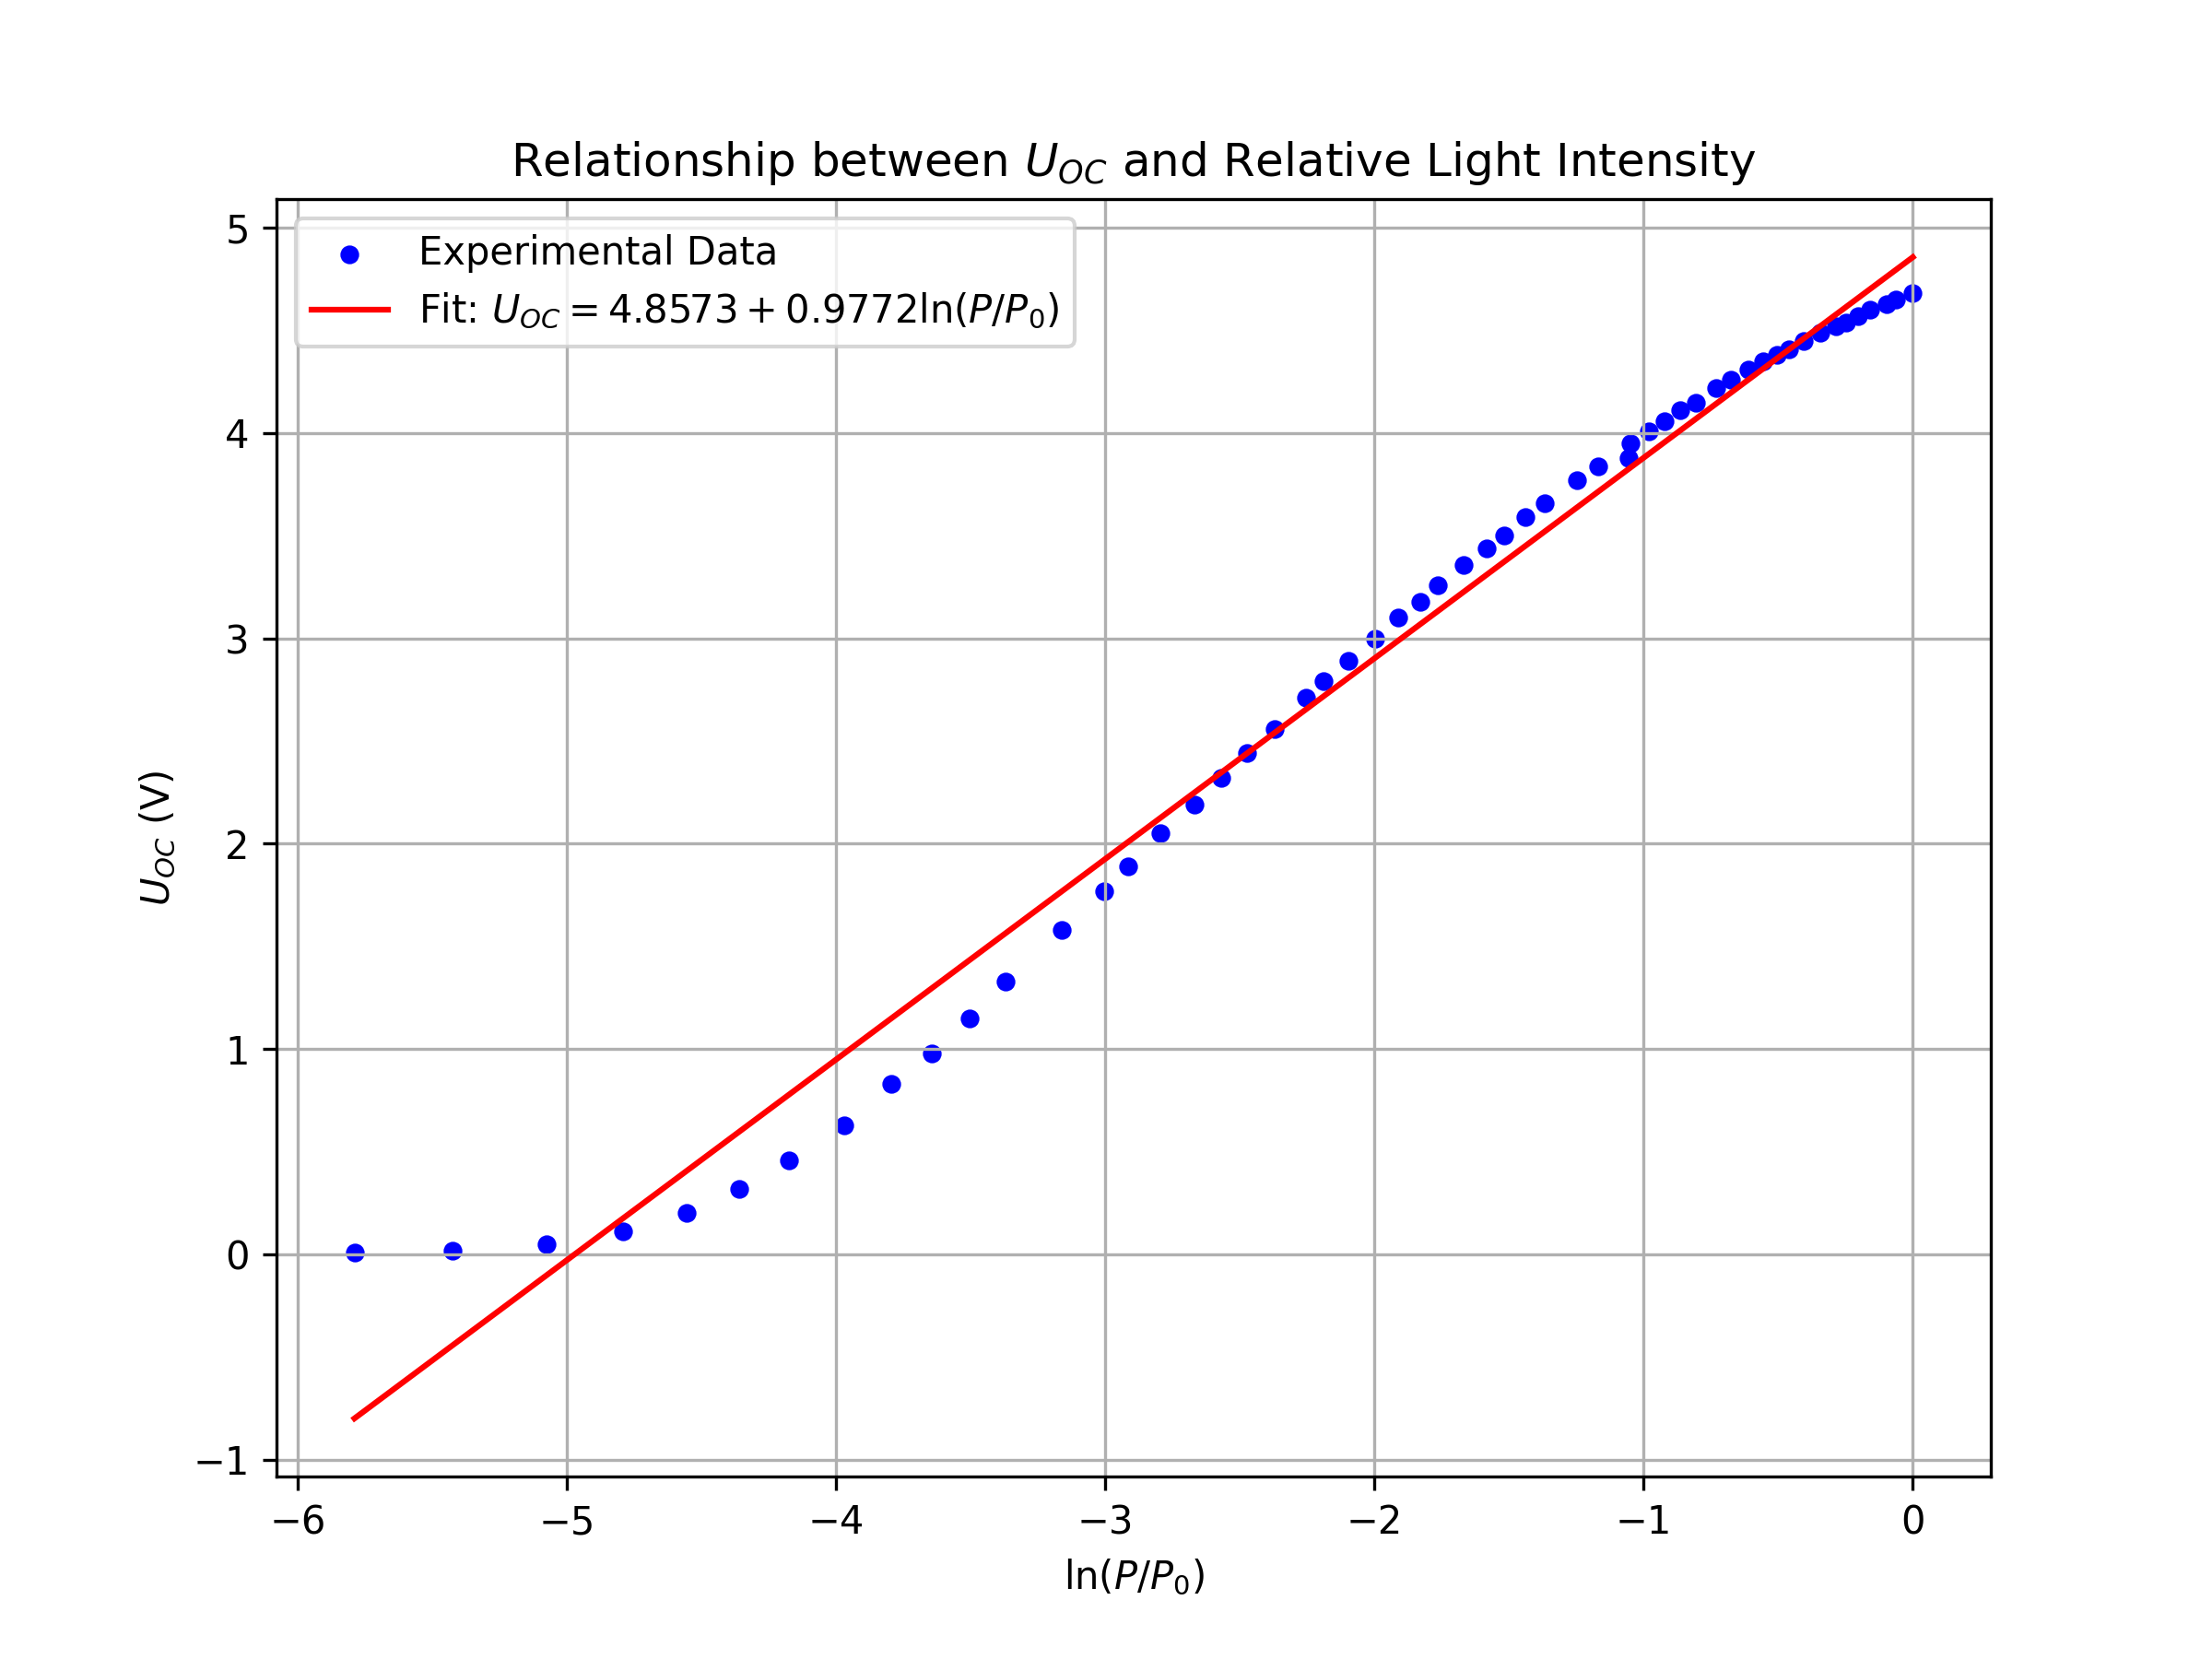
\includegraphics[width=0.7\textwidth]{fig_experiment4.png}
    \caption{开路电压 $U_{OC}$ 与相对光强对数 $\ln(P/P_0)$ 的关系曲线及拟合}
    \label{fig:uoc_lnp}
\end{figure}

线性拟合方程为：
\begin{equation}
    U_{OC} = 4.8573 + 0.9772 \cdot \ln\left(\frac{P_i}{P_0}\right)
\end{equation}
拟合结果显示 $U_{OC}$ 与 $\ln(P_i/P_0)$ 呈现良好的线性关系，验证了开路电压随光强对数增长的规律。

\subsection{短路电流 $I_{SC}$ 与相对光强的关系}


\begin{table}[htbp]
    \centering
    \caption{短路电流测量原始数据记录表}
    \begin{tabular}{cc|cc|cc}
        \toprule
        $U_0 / \text{V}$ & $U_2 / \text{mV}$ & $U_0 / \text{V}$ & $U_2 / \text{mV}$ & $U_0 / \text{V}$ & $U_2 / \text{mV}$ \\
        \midrule
        2.11 & 0.1 & 4.59 & 3.0 & 5.78 & 6.3 \\
        2.60 & 0.3 & 5.09 & 4.2 & 6.16 & 7.4 \\
        3.09 & 0.7 & 5.60 & 5.6 & 6.35 & 8.2 \\
        3.62 & 1.3 &      &      & 6.48 & 8.6 \\
        4.11 & 2.0 &      &      &      &     \\
        \bottomrule
    \end{tabular}
\end{table}

\textbf{数据处理结果：}

根据实验三定标得到的经验公式 $P_{\text{光强}} = 0.5930 \cdot U_0^{2.7030}$ 计算光强，以最大光强 $P_0$ 为基准计算相对光强 $P_i/P_0$。短路电流 $I_{SC}$ 由取样电阻两端电压 $U_2$ 计算得到，即 $I_{SC} = U_2 / 10 \, (\text{mA})$。计算结果如表\ref{tab:isc_process}所示。

\begin{table}[htbp]
    \centering
    \caption{短路电流与相对光强关系计算表}
    \label{tab:isc_process}
    \begin{tabular}{cccc}
        \toprule
        $U_0 / \text{V}$ & $U_2 / \text{mV}$ & $P_i/P_0$ & $I_{SC} / \text{mA}$ \\
        \midrule
        2.11 & 0.1 & 0.048 & 0.01 \\
        2.60 & 0.3 & 0.085 & 0.03 \\
        3.09 & 0.7 & 0.135 & 0.07 \\
        3.62 & 1.3 & 0.207 & 0.13 \\
        4.11 & 2.0 & 0.292 & 0.20 \\
        4.59 & 3.0 & 0.394 & 0.30 \\
        5.09 & 4.2 & 0.521 & 0.42 \\
        5.60 & 5.6 & 0.674 & 0.56 \\
        5.78 & 6.3 & 0.734 & 0.63 \\
        6.16 & 7.4 & 0.872 & 0.74 \\
        6.35 & 8.2 & 0.947 & 0.82 \\
        6.48 & 8.6 & 1.000 & 0.86 \\
        \bottomrule
    \end{tabular}
\end{table}

以相对光强 $P_i/P_0$ 为横坐标，短路电流 $I_{SC}$ 为纵坐标绘制关系曲线，如图\ref{fig:isc_p}所示。

\begin{figure}[htbp]
    \centering
    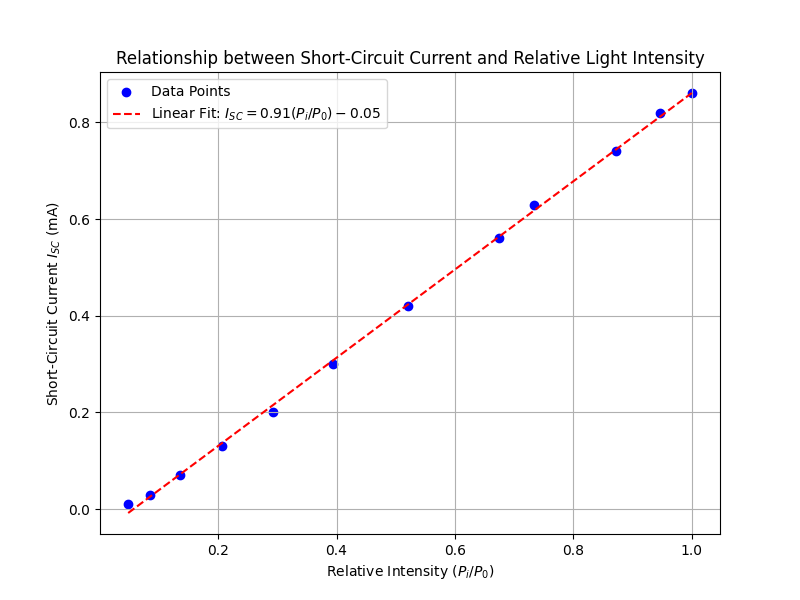
\includegraphics[width=0.7\textwidth]{fig_experiment5_SC.png}
    \caption{短路电流 $I_{SC}$ 与相对光强 $P_i/P_0$ 的关系曲线及拟合}
    \label{fig:isc_p}
\end{figure}

使用线性函数对数据进行拟合，拟合方程为：
\begin{equation}
    I_{SC} = 0.9129 \cdot \left(\frac{P_i}{P_0}\right) - 0.0520
\end{equation}
拟合结果表明，短路电流 $I_{SC}$ 与相对光强 $P_i/P_0$ 呈现良好的线性关系，验证了短路电流随光强线性增长的规律。

\subsection{反向偏压状态下硅光电池的光电特性}

\textbf{采样电阻：$R_{\text{取样}} = 10\,\Omega$}

\begin{table}[htbp]
    \centering
    \caption{不同光源电压下反向偏置伏安特性原始数据表}
    \begin{tabular}{c|c|c|c}
        \toprule
        & $U_0 = 2\,\text{V}$ & $U_0 = 3\,\text{V}$ & $U_0 = 4\,\text{V}$ \\
        \cmidrule(lr){2-2} \cmidrule(lr){3-3} \cmidrule(lr){4-4}
        $U_1 / \text{V}$ & $U_2 / \text{mV}$ & $U_2 / \text{mV}$ & $U_2 / \text{mV}$ \\
        \midrule
        0.0  & 0.1 & 0.6 & 2.0 \\
        0.5  & 0.1 & 0.7 & 2.0 \\
        1.0  & 0.1 & 0.7 & 2.1 \\
        1.5  & 0.1 & 0.8 & 2.2 \\
        2.0  & 0.1 & 0.8 & 2.3 \\
        2.5  & 0.1 & 0.9 & 2.4 \\
        3.0  & 0.1 & 0.9 & 2.6 \\
        3.5  & 0.1 & 1.0 & 2.8 \\
        4.0  & 0.2 & 1.0 & 2.9 \\
        4.5  & 0.1 & 1.1 & 2.9 \\
        5.0  & 0.2 & 1.2 & 3.0 \\
        5.5  & 0.2 & 1.3 & 3.2 \\
        6.0  & 0.2 & 1.4 & 3.5 \\
        6.5  & 0.2 & 1.4 & 3.8 \\
        \bottomrule
    \end{tabular}
\end{table}

\textbf{数据处理结果：}

根据测量数据，计算流过硅光电池的电流 $I = U_2 / 10 \, (\text{mA})$ 和电池两端电压 $U = U_1 - U_2 \cdot 10^{-3} \, (\text{V})$。计算结果如表\ref{tab:reverse_process}所示。由于 $U_2$ 远小于 $U_1$，电池两端反向偏压 $U$ 数值上近似等于电源电压 $U_1$。

\begin{table}[htbp]
    \centering
    \caption{反向偏置状态下电压与电流计算表}
    \label{tab:reverse_process}
    \begin{tabular}{c|cc|cc|cc}
        \toprule
        $U_1 / \text{V}$ & \multicolumn{2}{c|}{$U_0 = 2\,\text{V}$} & \multicolumn{2}{c|}{$U_0 = 3\,\text{V}$} & \multicolumn{2}{c}{$U_0 = 4\,\text{V}$} \\
        \cmidrule(lr){2-3} \cmidrule(lr){4-5} \cmidrule(lr){6-7}
        & $U / \text{V}$ & $I / \text{mA}$ & $U / \text{V}$ & $I / \text{mA}$ & $U / \text{V}$ & $I / \text{mA}$ \\
        \midrule
        0.0 & 0.00 & 0.01 & 0.00 & 0.06 & 0.00 & 0.20 \\
        0.5 & 0.50 & 0.01 & 0.50 & 0.07 & 0.50 & 0.20 \\
        1.0 & 1.00 & 0.01 & 1.00 & 0.07 & 1.00 & 0.21 \\
        1.5 & 1.50 & 0.01 & 1.50 & 0.08 & 1.50 & 0.22 \\
        2.0 & 2.00 & 0.01 & 2.00 & 0.08 & 2.00 & 0.23 \\
        2.5 & 2.50 & 0.01 & 2.50 & 0.09 & 2.50 & 0.24 \\
        3.0 & 3.00 & 0.01 & 3.00 & 0.09 & 3.00 & 0.26 \\
        3.5 & 3.50 & 0.01 & 3.50 & 0.10 & 3.50 & 0.28 \\
        4.0 & 4.00 & 0.02 & 4.00 & 0.10 & 4.00 & 0.29 \\
        4.5 & 4.50 & 0.01 & 4.50 & 0.11 & 4.50 & 0.29 \\
        5.0 & 5.00 & 0.02 & 5.00 & 0.12 & 5.00 & 0.30 \\
        5.5 & 5.50 & 0.02 & 5.50 & 0.13 & 5.50 & 0.32 \\
        6.0 & 6.00 & 0.02 & 6.00 & 0.14 & 6.00 & 0.35 \\
        6.5 & 6.50 & 0.02 & 6.50 & 0.14 & 6.50 & 0.38 \\
        \bottomrule
    \end{tabular}
\end{table}

以电池两端实际电压 $U$ 为横坐标，电流 $I$ 为纵坐标，绘制不同光强（$U_0$）下的 $I-U$ 伏安特性曲线，如图\ref{fig:reverse_iv}所示。

\begin{figure}[htbp]
    \centering
    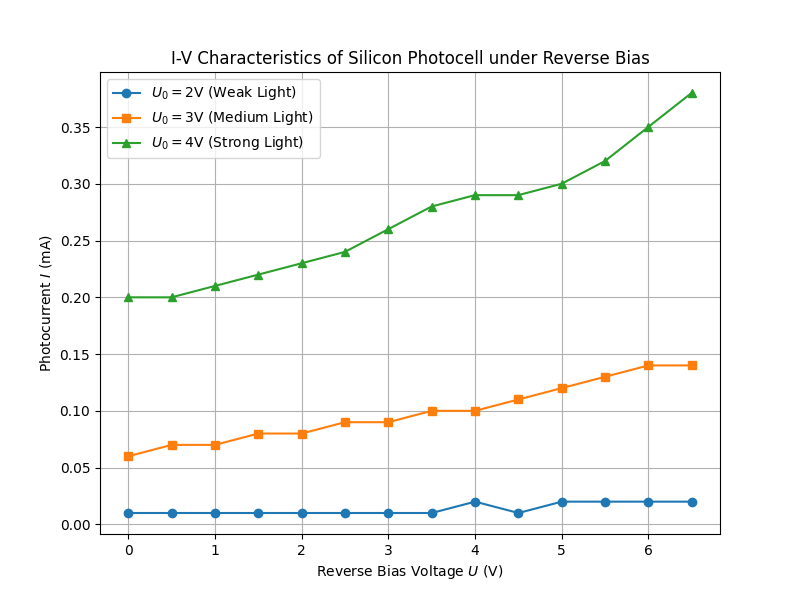
\includegraphics[width=0.7\textwidth]{fig_experiment6_reverse.png}
    \caption{反向偏压下硅光电池的伏安特性曲线}
    \label{fig:reverse_iv}
\end{figure}

从图中可以看出，在反向偏压状态下，硅光电池的电流随电压变化较小（尤其在低光强下近似饱和），表现出恒流源的特性。电流的大小主要取决于入射光强，随着光强（$U_0$）增加，反向饱和电流明显增大。

\section{实验总结}

通过本次实验，我们系统地测量并分析了硅光电池在无光照和光照条件下的基本光电特性，验证了光生伏特效应的物理机制。主要结论如下：

\begin{enumerate}
    \item \textbf{无光照伏安特性（暗特性）：}
    在无光照条件下，硅光电池表现出与普通半导体二极管一致的单向导电性。实验测得其正向电流随电压呈指数增长，拟合公式为 $I = 3.22 \times 10^{-5} \cdot e^{2.27 U}$，验证了 PN 结的整流特性。

    \item \textbf{光照下的负载特性：}
    在恒定光强下，硅光电池的输出功率随负载电阻的变化呈现先增大后减小的趋势。实验测得在当前光强下的最大输出功率 $P_m = 2.60\,\text{mW}$，对应的最佳负载电阻 $R_m = 6.77\,\text{k}\Omega$。计算得到的填充因子 $FF \approx 0.72$，表明该硅光电池具有较好的输出特性和光电转换效率。

    \item \textbf{开路电压与短路电流的光电响应：}
    实验定量验证了硅光电池两个关键参数与入射光强的函数关系：
    \begin{itemize}
        \item \textbf{开路电压 $U_{OC}$：} 随相对光强的对数线性增加。拟合关系 $U_{OC} \propto \ln(P_i/P_0)$ 得到验证，符合 PN 结光生电动势理论公式。
        \item \textbf{短路电流 $I_{SC}$：} 随相对光强呈现良好的线性增长关系。拟合方程为 $I_{SC} = 0.9129 \cdot (P_i/P_0) - 0.0520$，表明短路电流是表征入射光强度的理想参数，这也是硅光电池可作为线性光传感器（如照度计）的物理基础。
    \end{itemize}

    \item \textbf{反向偏压特性：}
    在反向偏置状态下，硅光电池表现出恒流源特性。光生电流几乎不随反向电压的变化而变化，而主要取决于入射光强的大小。这说明在光电检测电路中，施加反向偏压可以提高响应速度且不影响光电流的大小，同时也验证了光电池作为有源器件（光电池模式）和无源器件（光电二极管模式）时的不同工作机制。
\end{enumerate}

综上所述，本实验圆满完成了各项测量任务，深入理解了硅光电池从“光信号”到“电信号”转换的线性与非线性规律，掌握了最大功率点的测定方法以及填充因子等性能参数的物理意义。

\section{思考题}

\begin{enumerate}
    \item \textbf{在现代的生活中，太阳能有哪些用途？较其他能源太阳能有什么优点？}
    \begin{itemize}
        \item \textbf{用途：} 光伏发电（屋顶太阳能板、大型荒漠电站）、航天器动力（人造卫星太阳能帆板）、太阳能热水器、太阳能路灯、便携式电子产品（太阳能计算器、充电宝）等。
        \item \textbf{优点：} 
            1. \textbf{可再生性：} 能量来源无穷无尽，无需担心枯竭；
            2. \textbf{环保性：} 使用过程中无污染物排放，无噪音，不产生温室气体；
            3. \textbf{分布广泛：} 不受地域限制，尤其适合偏远或电网无法覆盖的地区；
            4. \textbf{维护成本低：} 太阳能电池组件通常寿命长，机械运动部件少。
    \end{itemize}

    \item \textbf{选取不同取样电阻 $1\,\Omega$、$10\,\Omega$、$100\,\Omega$ 对实验的测量结果分别有什么影响？（对实验数据的精度，以及实验数据的准确度有影响）}
    \begin{itemize}
        \item \textbf{对准确度的影响：} 取样电阻相当于接入电路的额外负载。在测量短路电流 $I_{SC}$ 时，理想情况下负载应为 0。
            \begin{itemize}
                \item $1\,\Omega$ 最接近理想短路状态，测得电流最接近真实的 $I_{SC}$，准确度最高；
                \item $100\,\Omega$ 电阻较大，会改变 PN 结两端的偏压，使其偏离短路点，导致测量值的准确度下降。
            \end{itemize}
        \item \textbf{对精度的影响：} 实验是通过测量 $U_2$ 后换算电流 $I = U_2 / R_{\text{取样}}$。
            \begin{itemize}
                \item 若取样电阻太小（如 $1\,\Omega$），在低光强下产生的电压 $U_2$ 会非常微弱，受电压表分辨率限制和背景噪声影响，读数相对误差大，精度较低；
                \item $10\,\Omega$ 或 $100\,\Omega$ 能产生较明显的电压信号，提高读数的分辨率和数据稳定性，即提高了精度。
            \end{itemize}
        \item \textbf{结论：} 实验中通常选取 $10\,\Omega$ 是为了在准确度（接近短路）和精度（信号足够强）之间取得平衡。
    \end{itemize}

    \item \textbf{实验中，电压表对电路有什么影响，如何减小影响？还有什么因素对实验有影响？}
    \begin{itemize}
        \item \textbf{电压表的影响：} 电压表具有有限的内阻 $R_V$，并联在电路中会产生“分流效应”，使得流经负载的实际电流减小，从而导致测量电压低于理论值。
        \item \textbf{减小方法：} 选用高内阻的数字电压表（通常内阻在 $10\,\text{M}\Omega$ 以上），使其分流作用可以忽略不计。
        \item \textbf{其他影响因素：} 
            1. \textbf{温度影响：} PN 结对温度敏感，长时间照射会导致电池升温，改变开路电压 $U_{OC}$ 和反向饱和电流 $I_0$；
            2. \textbf{背景光干扰：} 实验室的室内照明或其他散射光会叠加在光源上，影响定标和测量结果；
            3. \textbf{光源稳定性：} 光源电压的波动会直接导致入射光强变化；
            4. \textbf{光路对准：} 光源与电池盒若未完全对准或垂直，会降低能量接收效率。
    \end{itemize}
\end{enumerate}

\newpage
\section{原始记录和预习实验报告}

\begin{figure}[htbp]
    \centering
    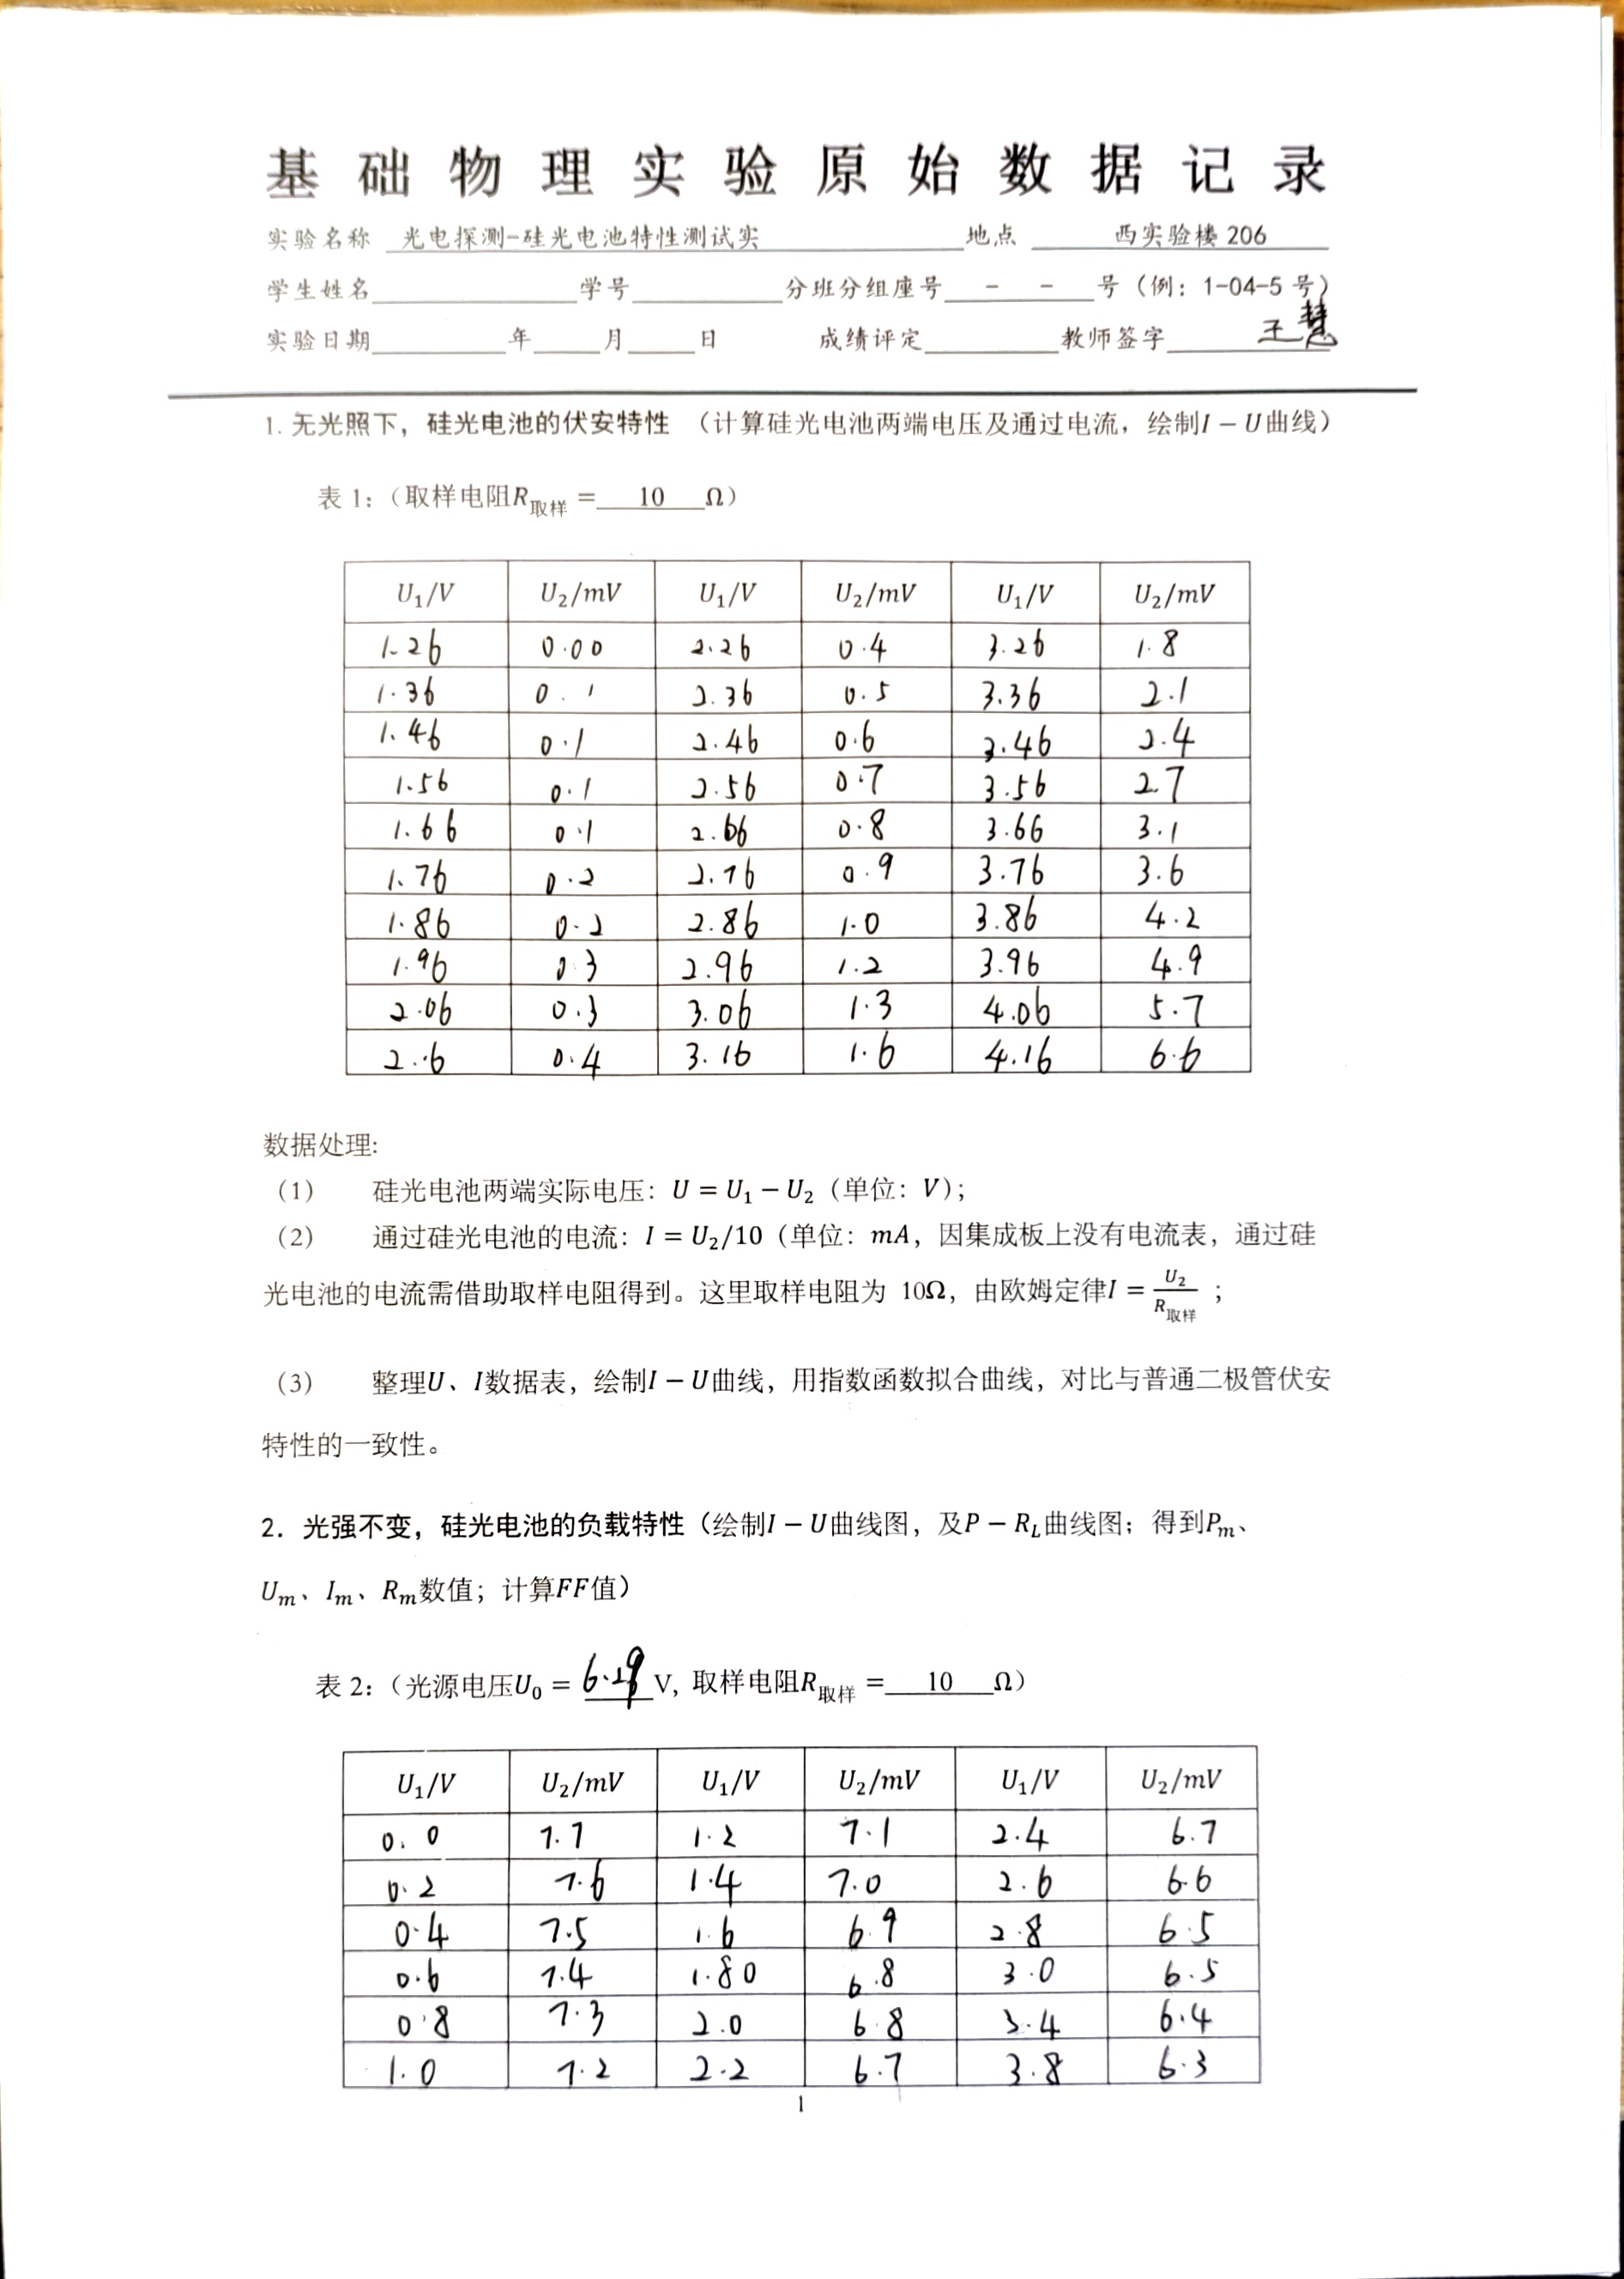
\includegraphics[width=0.9\textwidth]{record_1_1.jpg}
    \caption{原始记录页 1}
\end{figure}

\begin{figure}[htbp]
    \centering
    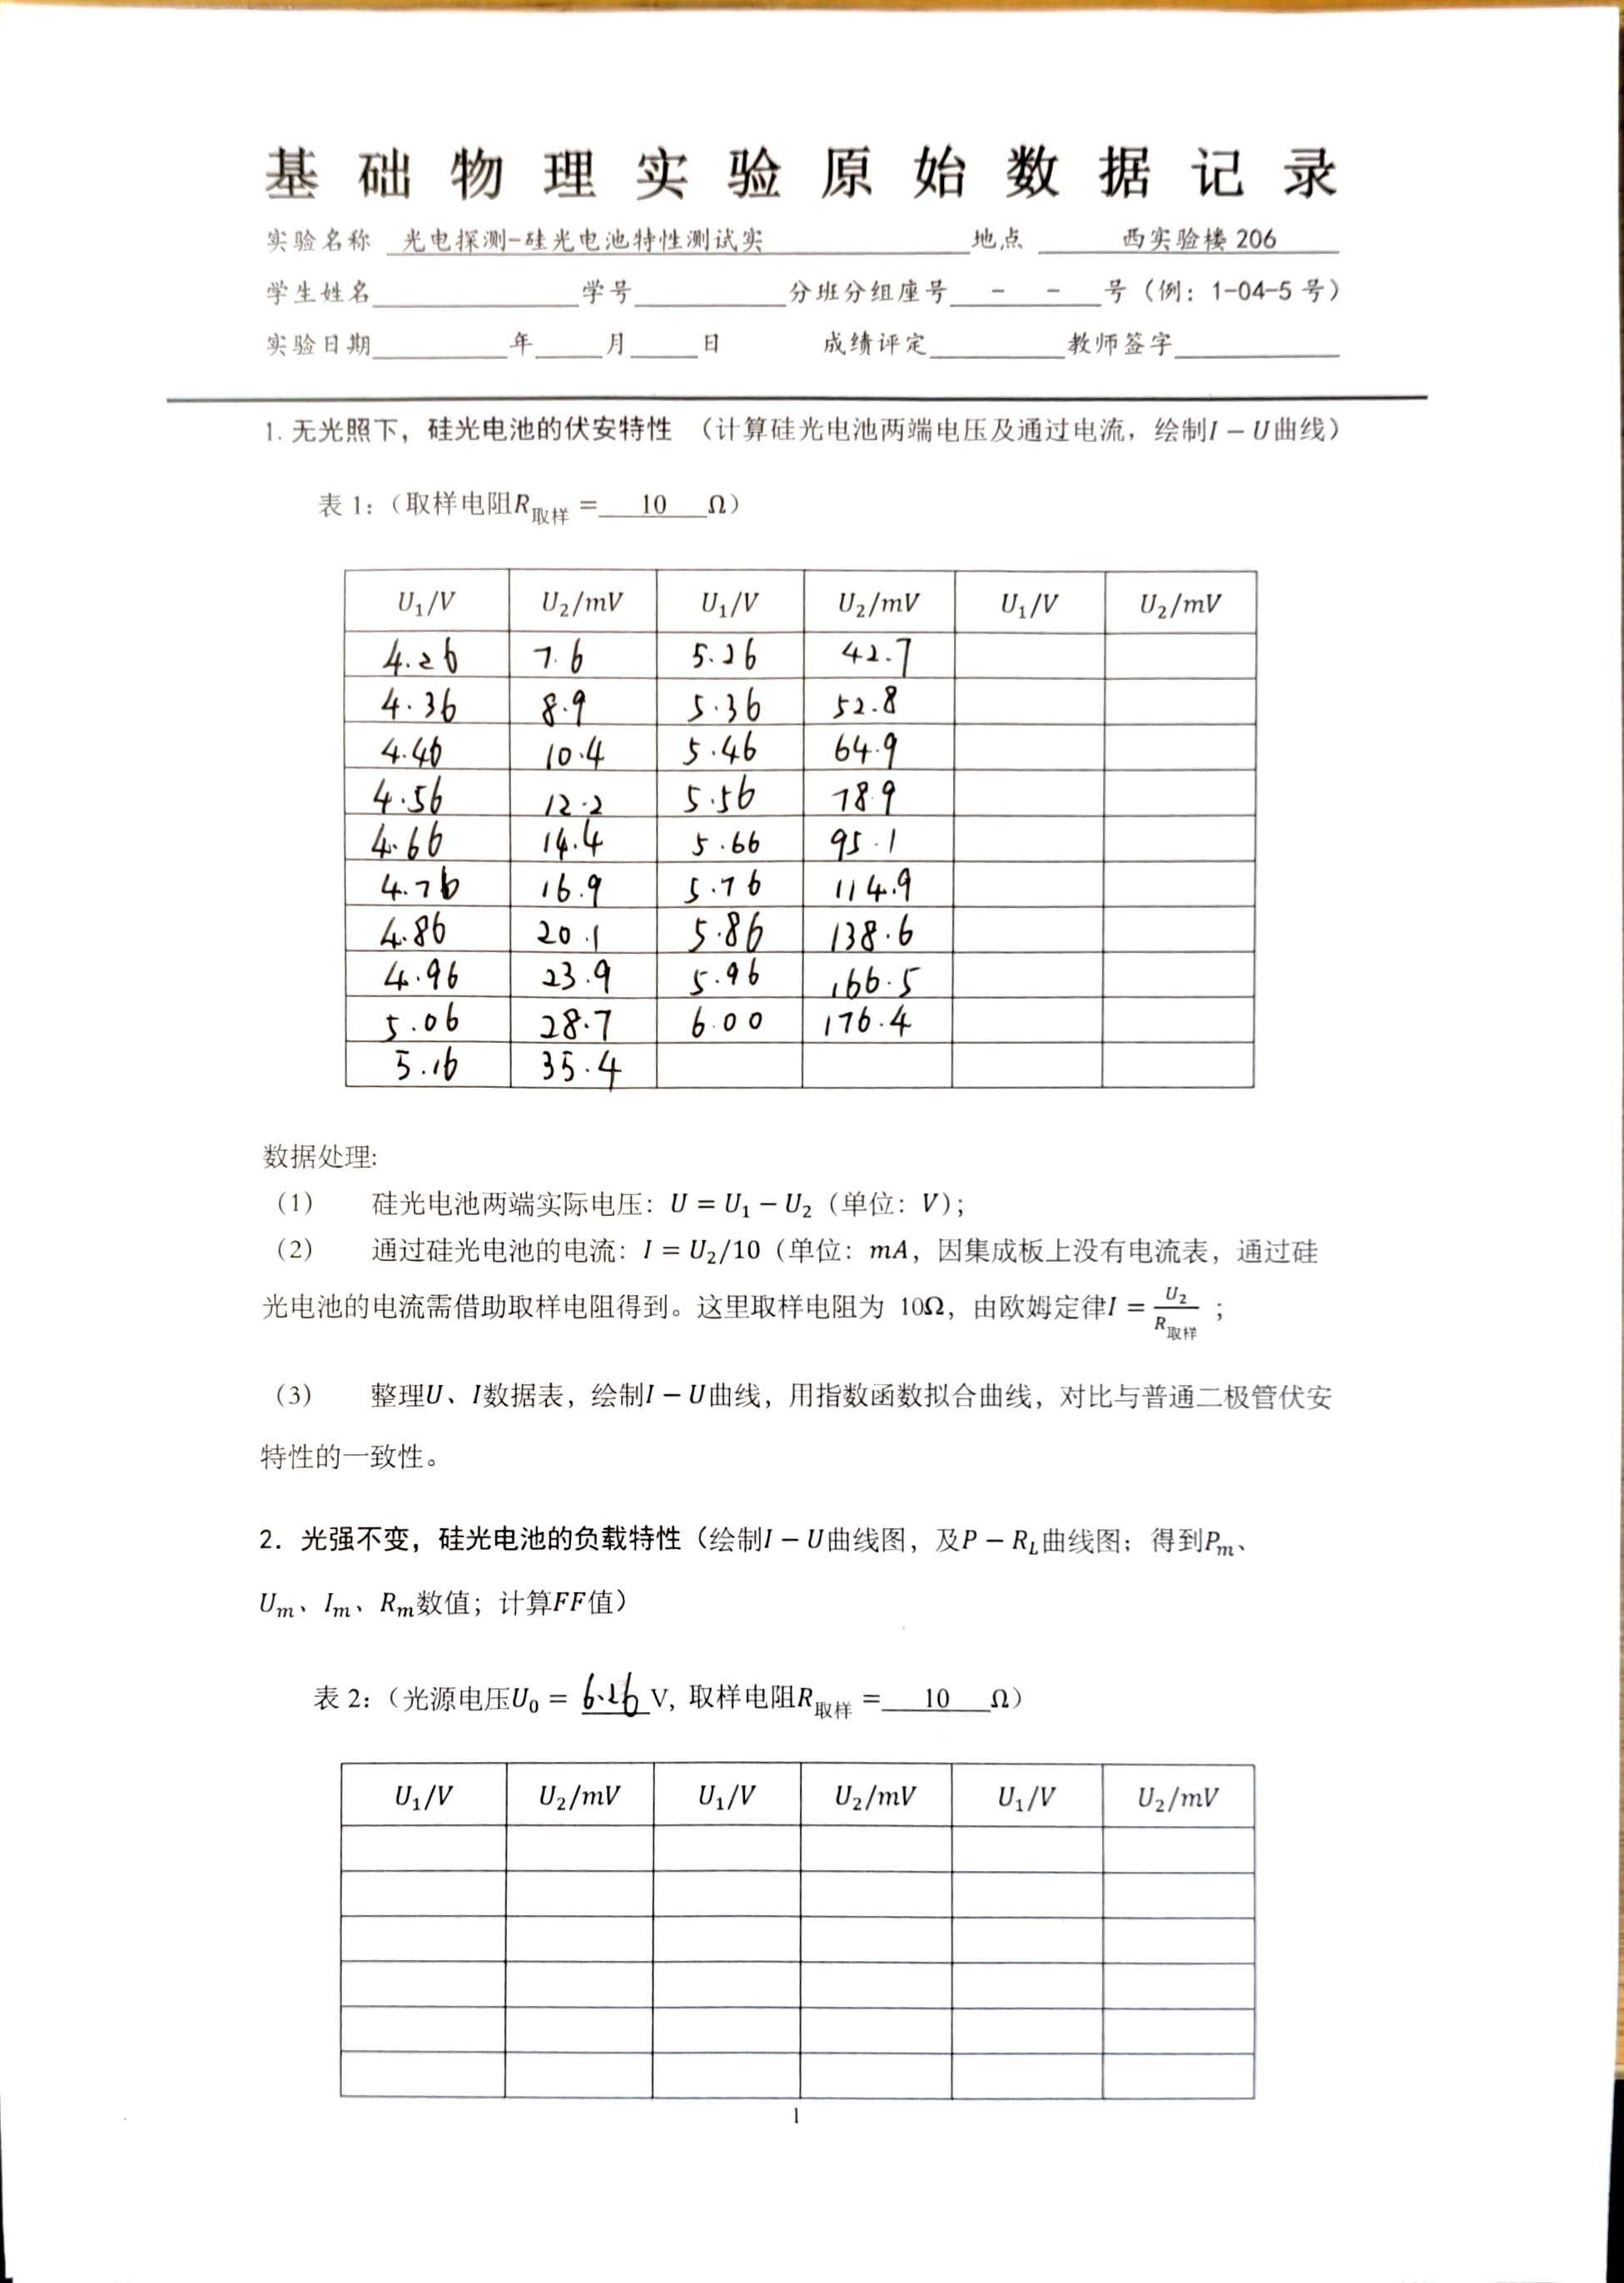
\includegraphics[width=0.9\textwidth]{record_1_2.jpg}
    \caption{原始记录页 2}
\end{figure}

\begin{figure}[htbp]
    \centering
    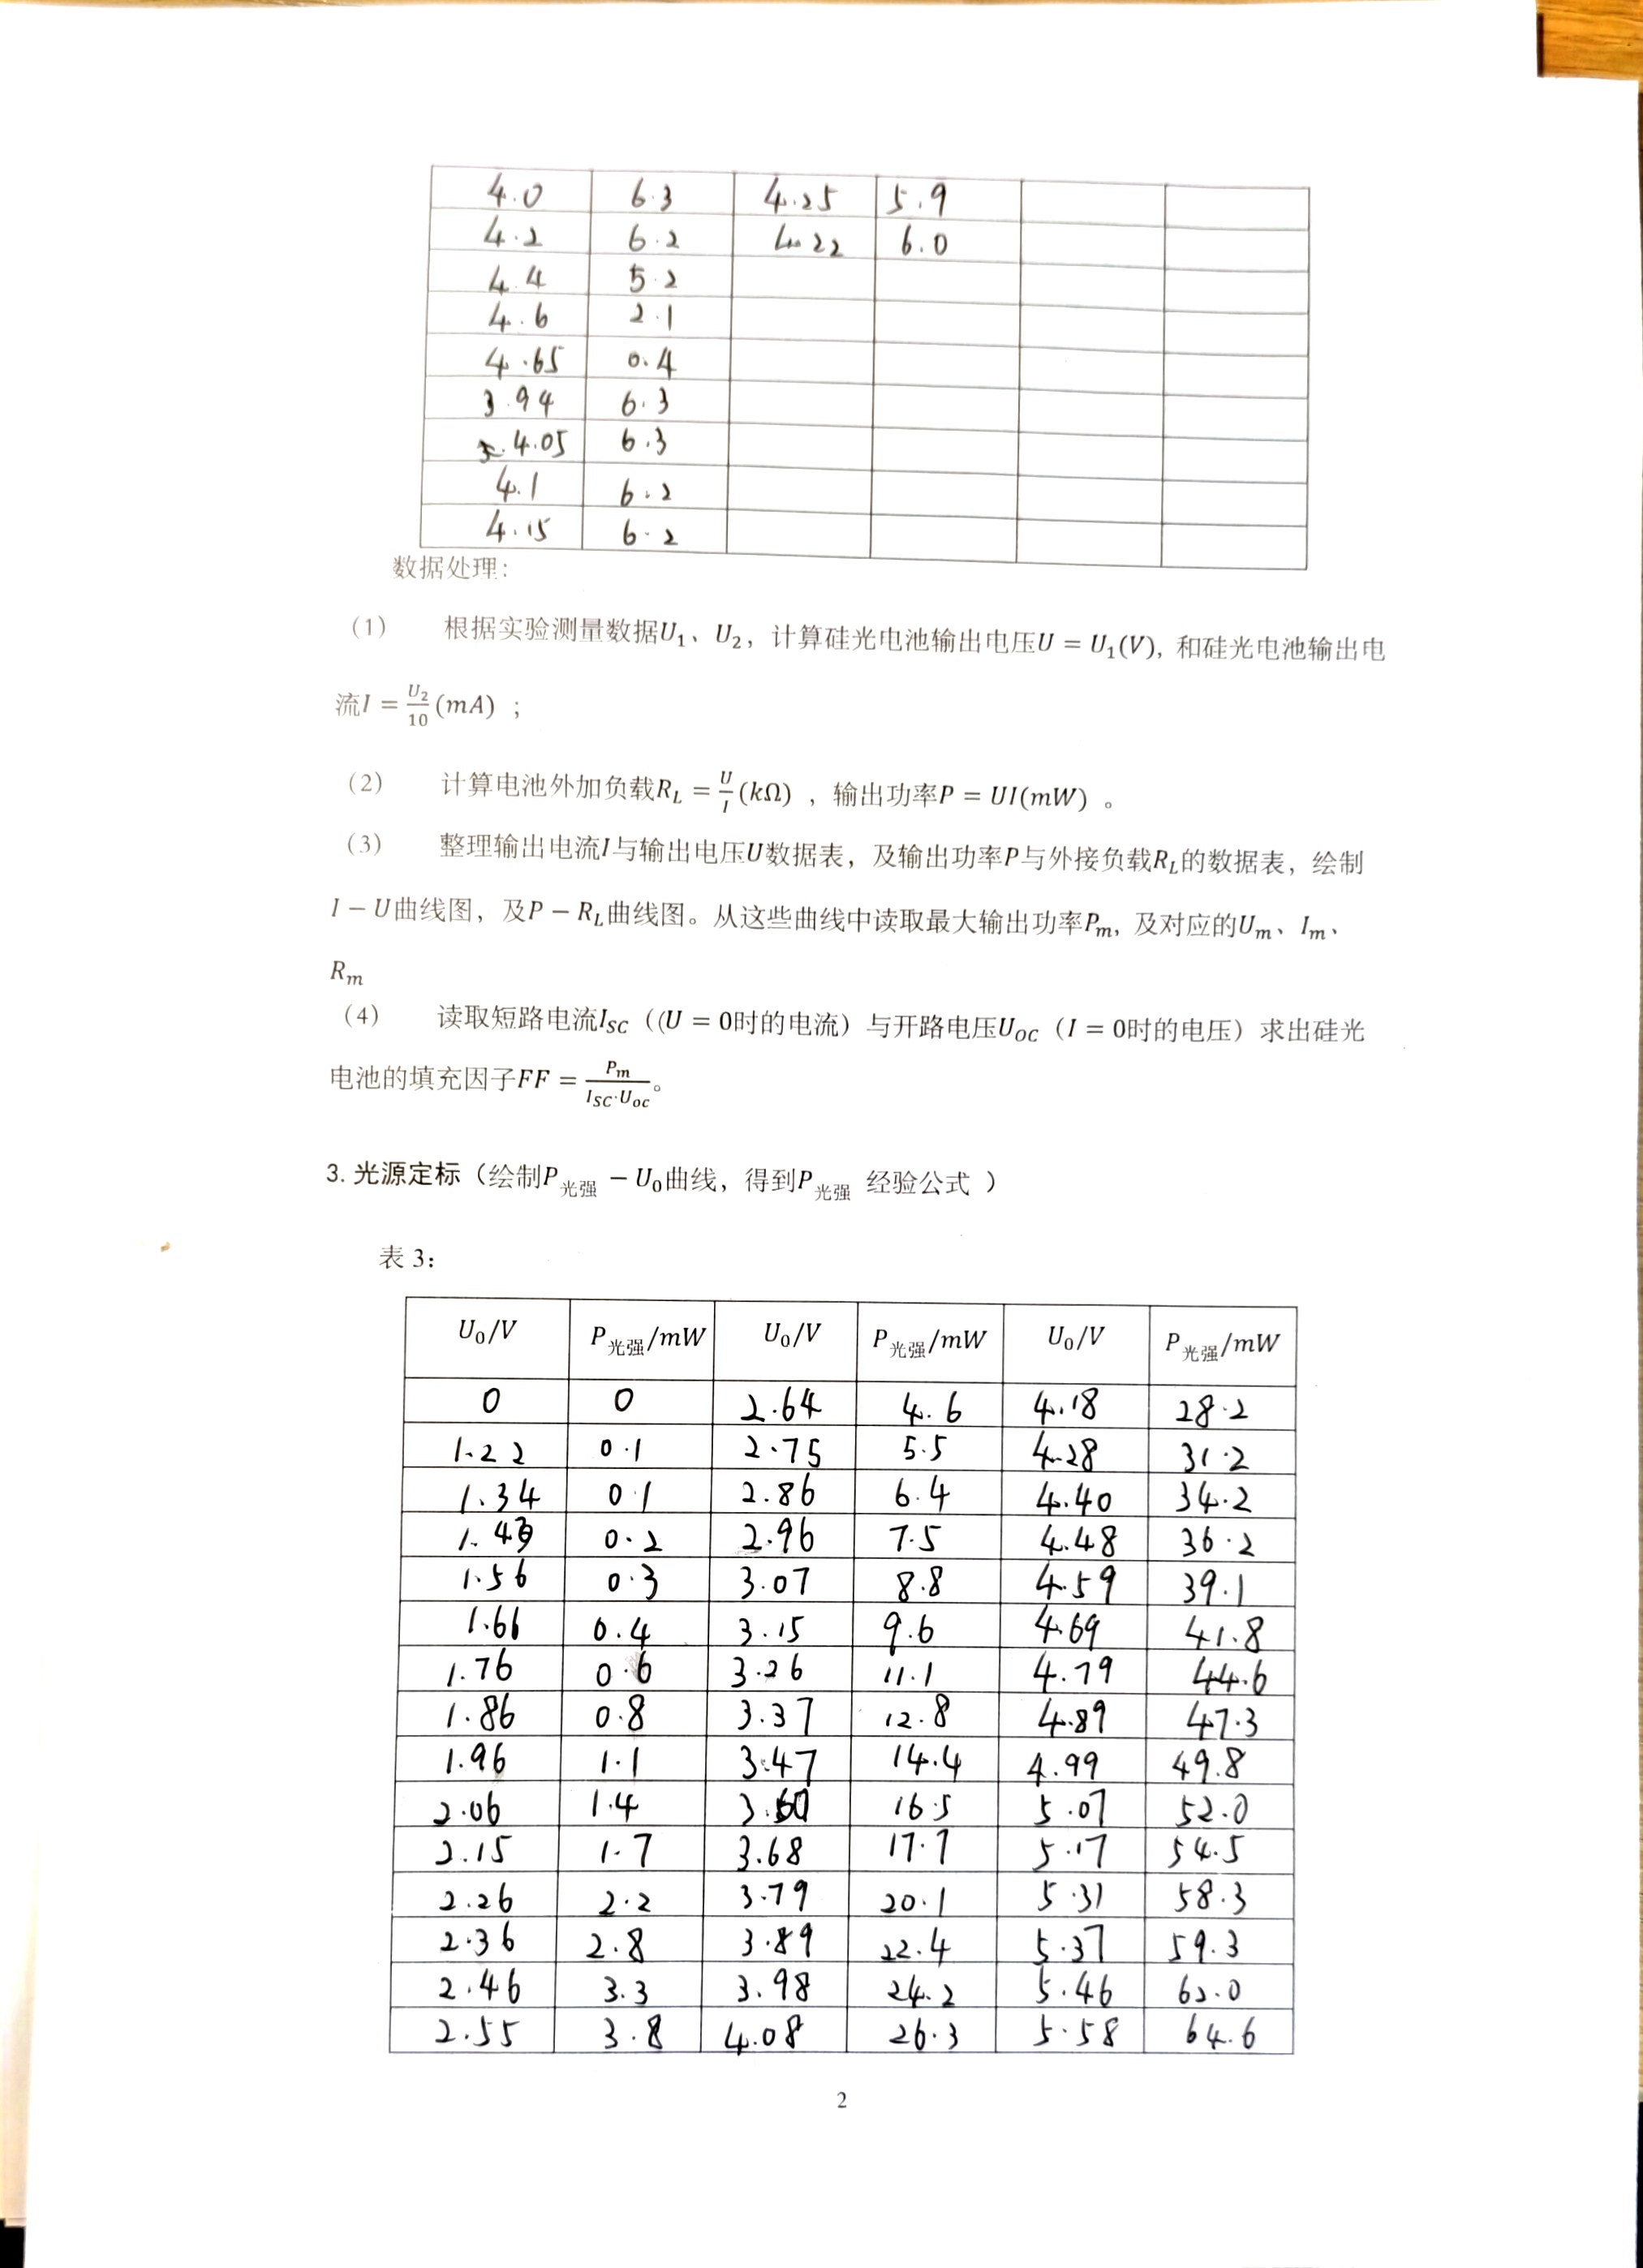
\includegraphics[width=0.9\textwidth]{record_2.jpg}
    \caption{原始记录页 3}
\end{figure}

\begin{figure}[htbp]
    \centering
    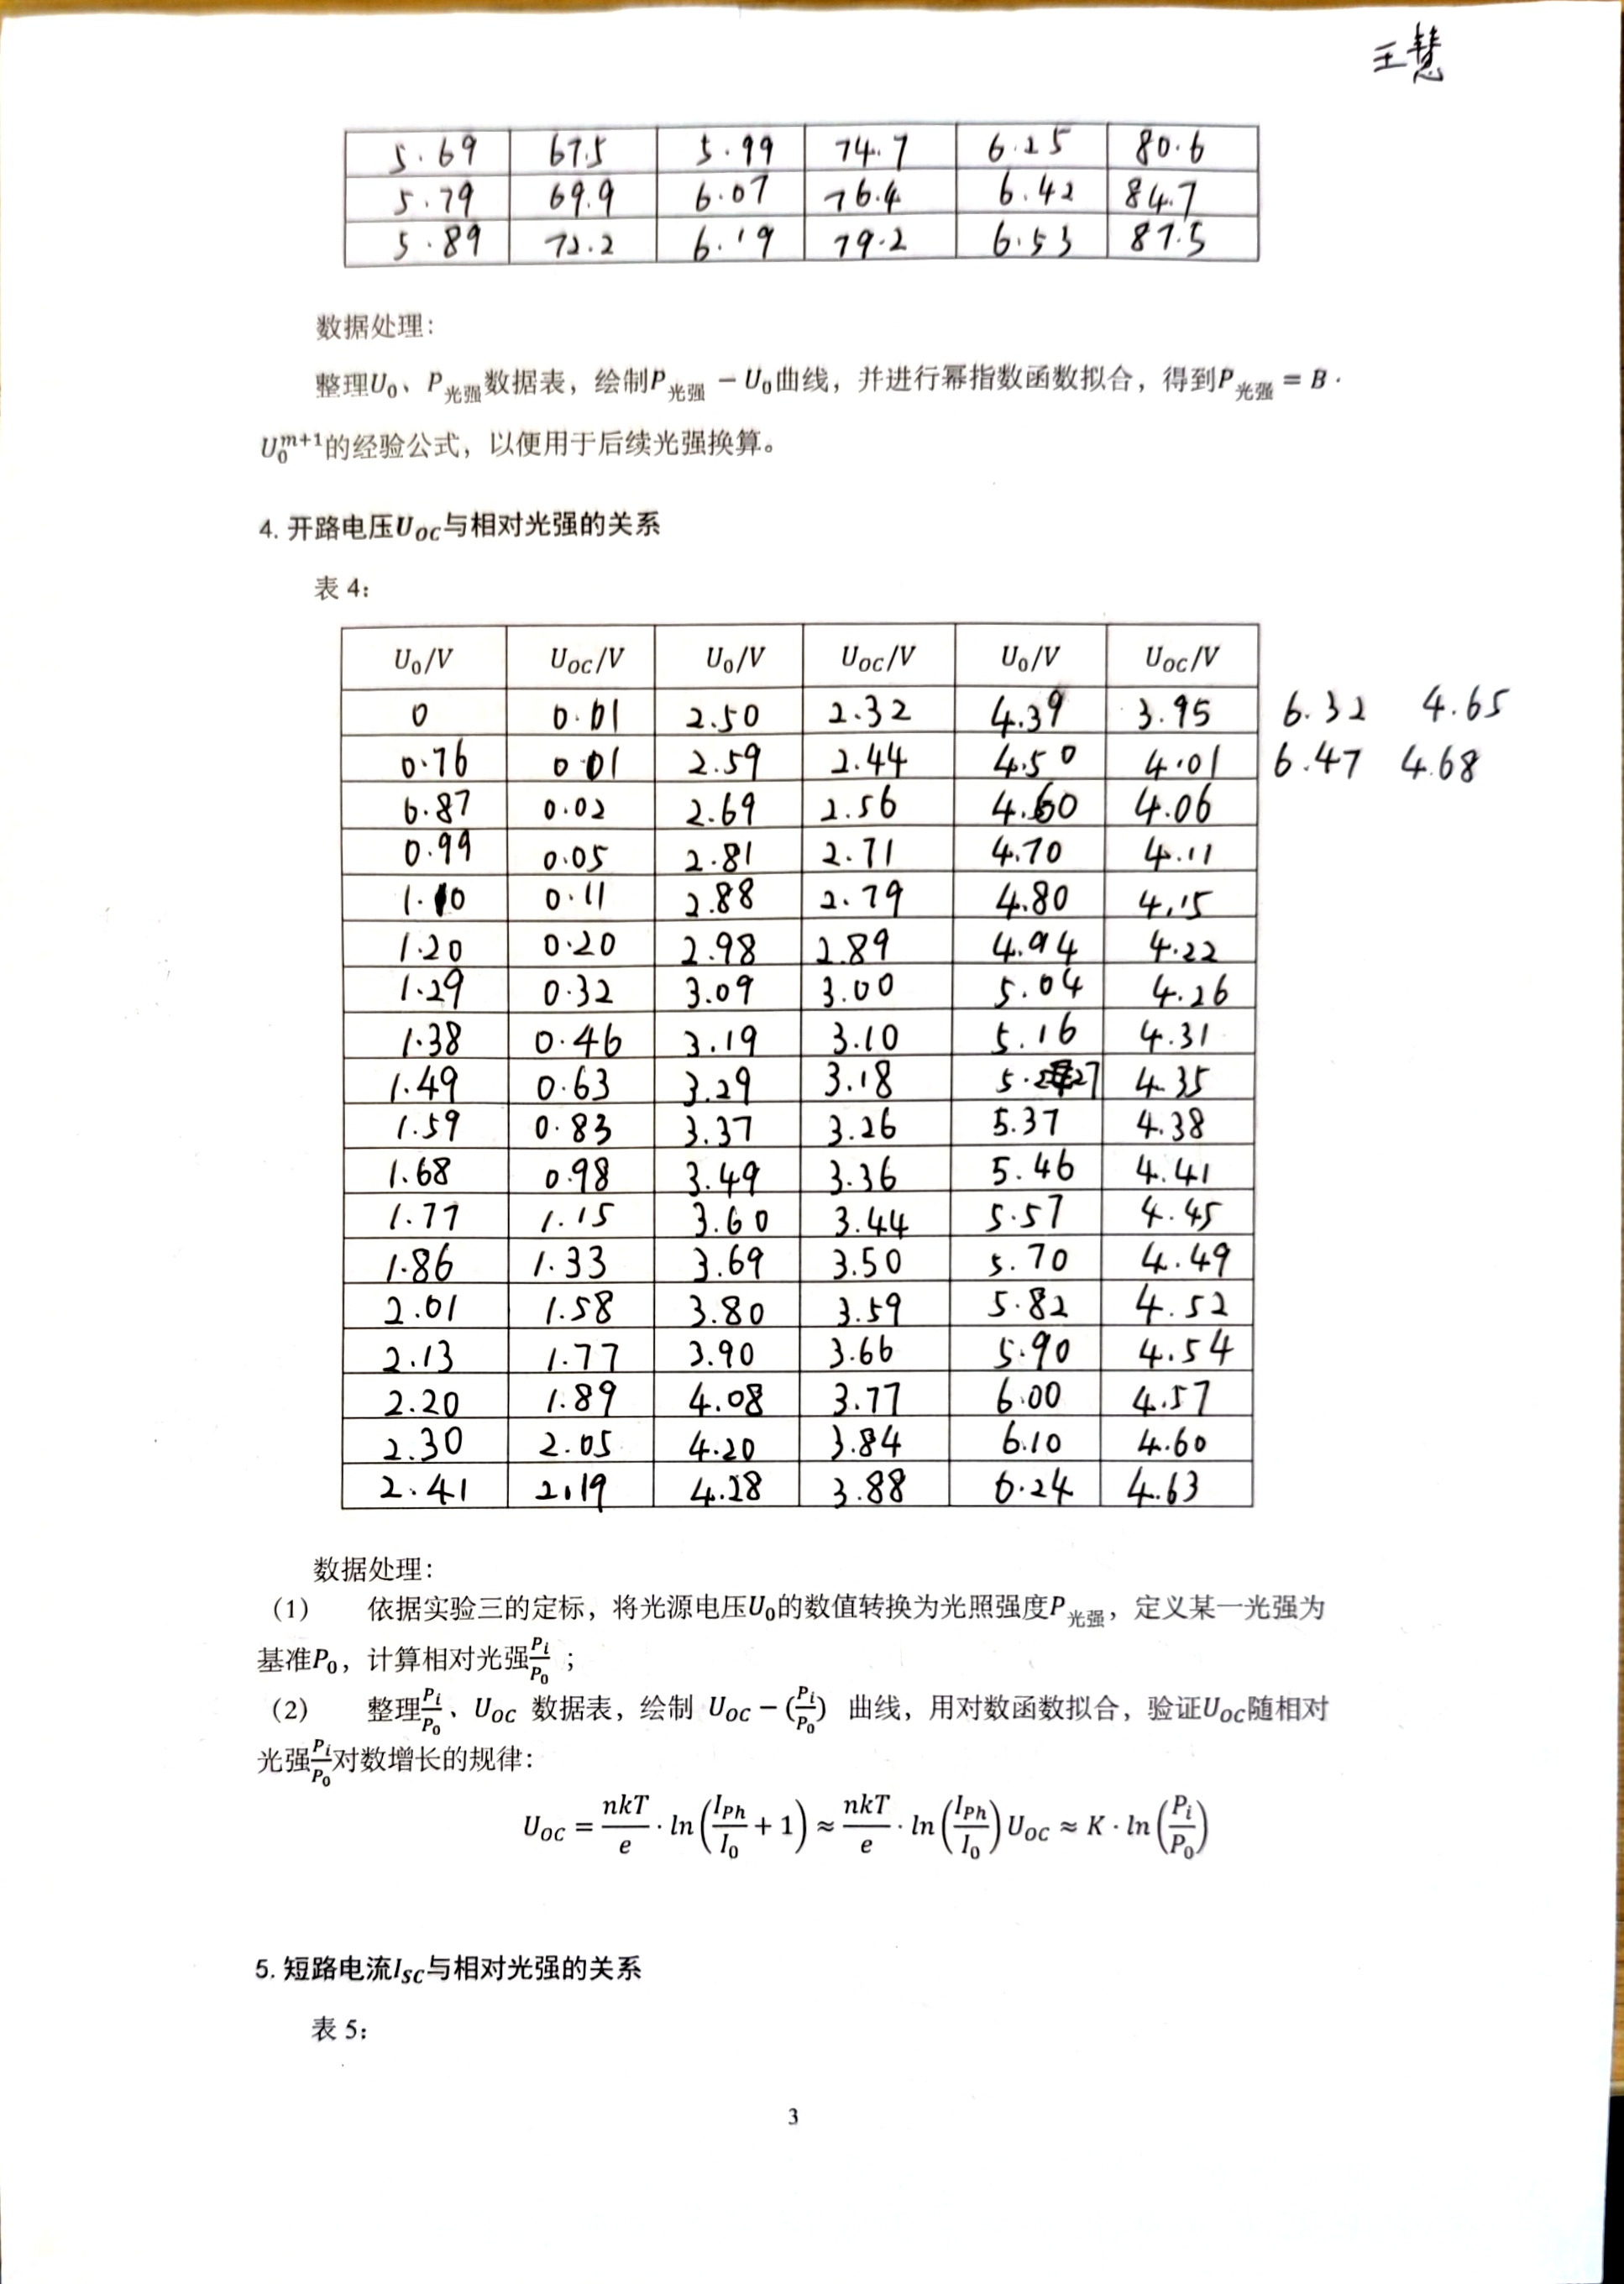
\includegraphics[width=0.9\textwidth]{record_3.jpg}
    \caption{原始记录页 4}
\end{figure}

\begin{figure}[htbp]
    \centering
    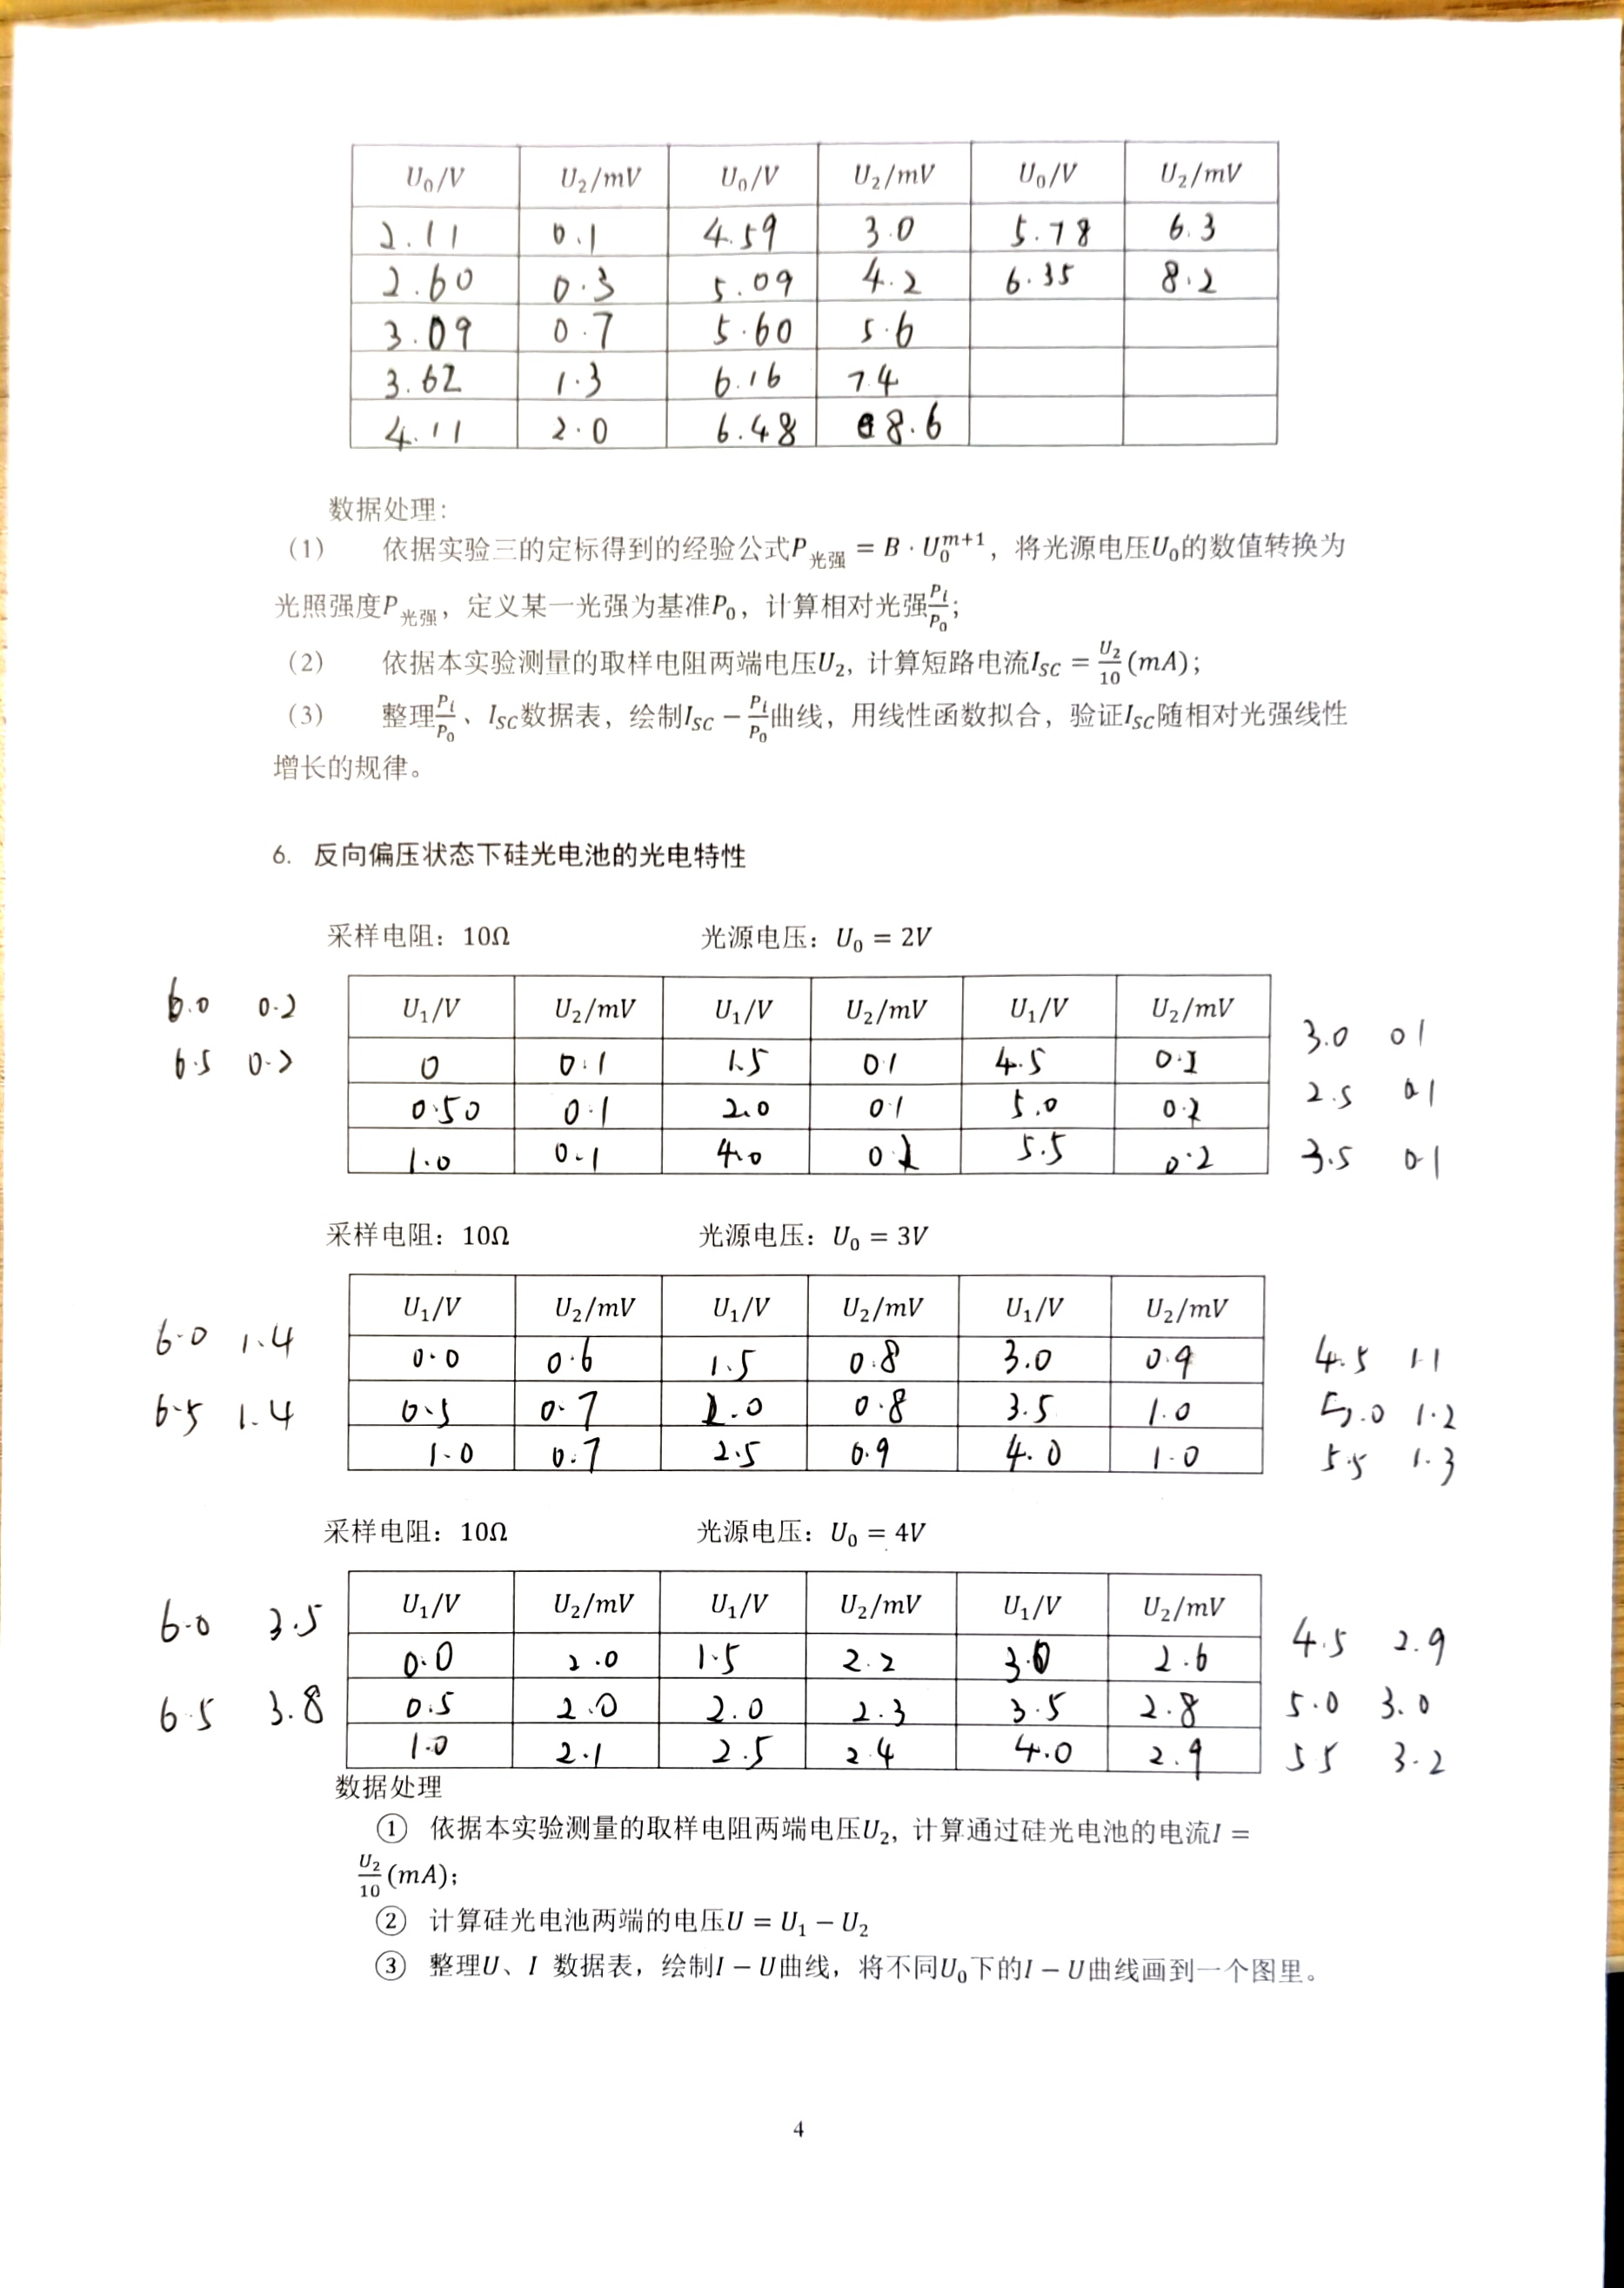
\includegraphics[width=0.9\textwidth]{record_4.jpg}
    \caption{原始记录页 5}
\end{figure}

\begin{figure}[htbp]pre
    \centering
    
\includegraphics[width=0.9\textwidth]{record_pre.jpg}
    \caption{预习实验报告}
\end{figure}

\end{document}